\documentclass{article}

% if you need to pass options to natbib, use, e.g.:
%     \PassOptionsToPackage{numbers, compress}{natbib}
% before loading neurips_2026

% The authors should use one of these tracks.
% Before accepting by the NeurIPS conference, select one of the options below.
% 0. "default" for submission
\usepackage{neurips_2026}
% the "default" option is equal to the "main" option, which is used for the Main Track with double-blind reviewing.
% 1. "main" option is used for the Main Track
%  \usepackage[main]{neurips_2026}
% 2. "position" option is used for the Position Paper Track
%  \usepackage[position]{neurips_2026}
% 3. "eandd" option is used for the Evaluations & Datasets Track
 % \usepackage[eandd]{neurips_2026}
 % if you need to opt-in for a single-blind submission in the E&D track:
 %\usepackage[eandd, nonanonymous]{neurips_2026}
% 4. "creativeai" option is used for the Creative AI Track
%  \usepackage[creativeai]{neurips_2026}
% 5. "sglblindworkshop" option is used for the Workshop with single-blind reviewing
 % \usepackage[sglblindworkshop]{neurips_2026}
% 6. "dblblindworkshop" option is used for the Workshop with double-blind reviewing
%  \usepackage[dblblindworkshop]{neurips_2026}

% After being accepted, the authors should add "final" behind the track to compile a camera-ready version.
% 1. Main Track
 % \usepackage[main, final]{neurips_2026}
% 2. Position Paper Track
%  \usepackage[position, final]{neurips_2026}
% 3. Evaluations & Datasets Track
 % \usepackage[eandd, final]{neurips_2026}
% 4. Creative AI Track
%  \usepackage[creativeai, final]{neurips_2026}
% 5. Workshop with single-blind reviewing
%  \usepackage[sglblindworkshop, final]{neurips_2026}
% 6. Workshop with double-blind reviewing
%  \usepackage[dblblindworkshop, final]{neurips_2026}
% Note. For the workshop paper template, both \title{} and \workshoptitle{} are required, with the former indicating the paper title shown in the title and the latter indicating the workshop title displayed in the footnote.
% For workshops (5., 6.), the authors should add the name of the workshop, "\workshoptitle" command is used to set the workshop title.
% \workshoptitle{WORKSHOP TITLE}

% "preprint" option is used for arXiv or other preprint submissions
 % \usepackage[preprint]{neurips_2026}

% to avoid loading the natbib package, add option nonatbib:
%    \usepackage[nonatbib]{neurips_2026}

\usepackage[utf8]{inputenc} % allow utf-8 input
\usepackage[T1]{fontenc}    % use 8-bit T1 fonts
\usepackage{hyperref}       % hyperlinks
\usepackage{url}            % simple URL typesetting
\usepackage{booktabs}       % professional-quality tables
\usepackage{amsfonts}       % blackboard math symbols
\usepackage{amsmath}        % align environment, etc.
\usepackage{nicefrac}       % compact symbols for 1/2, etc.
\usepackage{microtype}      % microtypography
\usepackage{xcolor}         % colors

\usepackage{graphicx}
\usepackage{subcaption}
\usepackage{float}
% Tables
\usepackage{tabularx}
\usepackage{multirow}
\usepackage{adjustbox}
% Plots
\usepackage{tikz}
\usepackage{enumitem}

\newcommand{\R}{\mathbb{R}}
\newcommand{\tzh}[1]{{\color{ForestGreen}{[Zhenghan: #1]}}}
% Note. For the workshop paper template, both \title{} and \workshoptitle{} are required, with the former indicating the paper title shown in the title and the latter indicating the workshop title displayed in the footnote. 
\title{Why Language Models Transfer to Time Series}


% The \author macro works with any number of authors. There are two commands
% used to separate the names and addresses of multiple authors: \And and \AND.
%
% Using \And between authors leaves it to LaTeX to determine where to break the
% lines. Using \AND forces a line break at that point. So, if LaTeX puts 3 of 4
% authors names on the first line, and the last on the second line, try using
% \AND instead of \And before the third author name.


\author{%
  David S.~Hippocampus\thanks{Use footnote for providing further information
    about author (webpage, alternative address)---\emph{not} for acknowledging
    funding agencies.} \\
  Department of Computer Science\\
  Cranberry-Lemon University\\
  Pittsburgh, PA 15213 \\
  \texttt{hippo@cs.cranberry-lemon.edu} \\
  % examples of more authors
  % \And
  % Coauthor \\
  % Affiliation \\
  % Address \\
  % \texttt{email} \\
  % \AND
  % Coauthor \\
  % Affiliation \\
  % Address \\
  % \texttt{email} \\
  % \And
  % Coauthor \\
  % Affiliation \\
  % Address \\
  % \texttt{email} \\
  % \And
  % Coauthor \\
  % Affiliation \\
  % Address \\
  % \texttt{email} \\
}


\begin{document}
\maketitle


\begin{abstract}
TODO
\end{abstract}


% ═══════════════════════════════════════════════════════════════
% The phenomenon: LLMs finetuned on time series match or beat domain-specific models.
% The question: Why should representations learned from text help with temporal data?
% We provide a concrete, mechanistic account.
%
% Our approach: investigate from first principles.
%   1. Establish that transfer actually happens and quantify it. -> raw benchmark perf of pretrain Vs random
%   2. Characterize what the pretrained model already has (what does it contain that is useful for time series?) Analysis on QWEN BASE as it pertains to transfer 
%   3. Characterize what changes during finetuning (what changes in the representation space?) Analsysi on QWEN finetuned Compare with the control (learning from scratch) comparison of QWEN finetuend w random
%   4. Conclusion on how transfer works 
%
% Preview the main finding: pretraining creates a geometric prior —
% a low-dimensional, smooth representation space with directions
% that naturally encode temporal dynamics. Transfer = selecting those directions.

\section{Introduction}
\label{sec:intro}

% The key contributions we make in this paper are as follows:
% \begin{itemize}[leftmargin=*]
%   \item TODO
% \end{itemize} 
% ═══════════════════════════════════════════════════════════════

% ═══════════════════════════════════════════════════════════════
% LLM-to-TS transfer literature
% See Alexis...bib, section TRANSFER for papers
% Share manifold hyptohesis
%   shared embedding paper? 
% Any works on cross domain representational analysis 

\section{Related work}
\label{sec:related_work}

\paragraph{Time-series foundation models (TSFMs).}
Models designed as general-purpose time series forecasters, trained on Large-scale multi-domain data
\begin{enumerate}
    \item Chronos \citep{}
    \item Lag-Llama \citep{}
    \item MOMENT \citep{}
    \item TimeGPT \citep{}
\end{enumerate}

\paragraph{LLM-to-time-series transfer.} 
Work that repurposes pretrained language models for time series, primary related work
\begin{enumerate}
    \item Are Language Models Actually Useful for Time Series Forecasting?" \citep{tan2024languagemodelsactuallyuseful}
    \item Time-LLM: Time Series Forecasting by Reprogramming Large Language Models \citep{jin2024timellmtimeseriesforecasting}
    \item Using Pre-trained LLMs for Multivariate Time Series Forecasting \citep{wolff2025usingpretrainedllmsmultivariate}
    \item isionTS: Visual Masked Autoencoders Are Free-Lunch Zero-Shot Time Series Forecasters \citep{chen2024visionts}
\end{enumerate}

\paragraph{Time Series Tokenization and Representation; LLM2TS continued}
\begin{enumerate}
    \item A Time Series is Worth 64 Words \citep{nie2023timeseriesworth64}
    \item Small Vocabularies, Big Gains \citep{roger2025smallvocabulariesbiggains}
\end{enumerate}

\paragraph{The Platonic Representation Hypothesis? Cross-Modal Geometry?}
Theoretical/empirical work on representation convergence to explain why might representations transfer across modalities -> Language to TS
\begin{enumerate}
    \item The Platonic Representation Hypothesis \citep{huh2024platonicrepresentationhypothesis}
    \item Harnessing the Universal Geometry of Embeddings \citep{jha2025harnessinguniversalgeometryembeddings}
    \item Training Large Language Models to Reason in a Continuous Latent Space \citep{hao2024traininglargelanguagemodels}
\end{enumerate}

\paragraph{Scaling Laws and Efficient Adaptation}
How (do we) do models scale and fine-tuning strategies interact with transfer
\begin{enumerate}
    \item Scaling Laws for Transfer \citep{hernandez2021scalinglawstransfer}
    \item Studies on when scaling hurts? \citep{}
    \item Parameter-efficient fine-tuning comparisons, LoRA vs Full vs Adapters \citep{}
\end{enumerate}
The findings that pretrained 0.6B matches random 4B implies a transfer multiplier of ~8x in effective parameters; io\_only regime (embedding + lm\_head only) indicate if the transfer is fully captured by the i/o layers → PEFT/LoRA
% ═══════════════════════════════════════════════════════════════

% ═══════════════════════════════════════════════════════════════
\section{Establishing Transfer Learning is Real}
\label{sec:transfer}

% Setup paragraph: models + data + tokenization
% TODO: Prateek/Alexis to add benchmark details

\paragraph{Setup.} All models share the Qwen3 architecture. We train pairs of \textbf{FT} (pretrained $\to$ finetuned on TS) and \textbf{RI} (random init $\to$ trained on TS) across multiple scales (0.6B, 1.7B, 4B) using the same TS training procedure (uniform binning, 512 bins, context length 512). All models are evaluated on GiftEval (46 datasets).

\paragraph{Main result.} FT consistently outperforms RI across scales and datasets.

% ── TABLE: Benchmark results across scales ──
% TODO: Fill with actual ND[0.5] numbers from Alexis's sweeps
\begin{table}[h]
\centering
\caption{ND[0.5] on GiftEval (lower is better). FT outperforms RI at all scales.}
\label{tab:benchmark}
\begin{tabular}{lcccc}
\toprule
Model & 0.6B & 1.7B & 4B \\
\midrule
FT (pretrained + TS)  & TODO & TODO & TODO \\
RI (random + TS)      & TODO & TODO & TODO \\
\midrule
$\Delta$ (FT $-$ RI)  & TODO & TODO & TODO \\
\bottomrule
\end{tabular}
\end{table}

\paragraph{Scaling interaction.} Pretrained 0.6B matches or exceeds random-init 4B, implying a transfer multiplier of $\sim$8$\times$ in effective parameters.

% ── FIGURE: Performance across scales ──
% TODO: Bar chart or line plot showing FT vs RI at each scale
% Source: Alexis's training runs

\paragraph{Finetuning regime comparison.} We compare full finetuning, LoRA, and IO-only (embedding + LM head only).
% TODO: Table showing that even IO-only captures substantial transfer
% This previews the low-rank story in Section~\ref{sec:finetuning}

% ═══════════════════════════════════════════════════════════════

% ═══════════════════════════════════════════════════════════════

\section{The Shared Manifold Hypothesis}
\label{sec:prior}

Having established the existence of transfer learning from LLMs to time series in Sec.~\ref{sec:transfer}, we now present a geometric explanation for why LLMs are such adept time series forecasters. Due to the recursive structure and statistical patterns exhibited by language \citep{ou2025identifying}, we theorize that pretrained language model representations already contain native temporal structures well suited for adaptation to time series data. In this section, we present several experiments demonstrating that LLMs do possess a manifold that is already compatible with time series forecasting, and that fine-tuning does not need to create new directions, it simply identifies and collapses time series representations onto the best pre-existing directions.

\subsection{A Linear Probe Reveals Latent Temporal Structure}
% ── FIGURE: Examples + Ablation side by side ──
\begin{figure}[!t]
\centering
\begin{subfigure}[t]{0.48\textwidth}
\centering
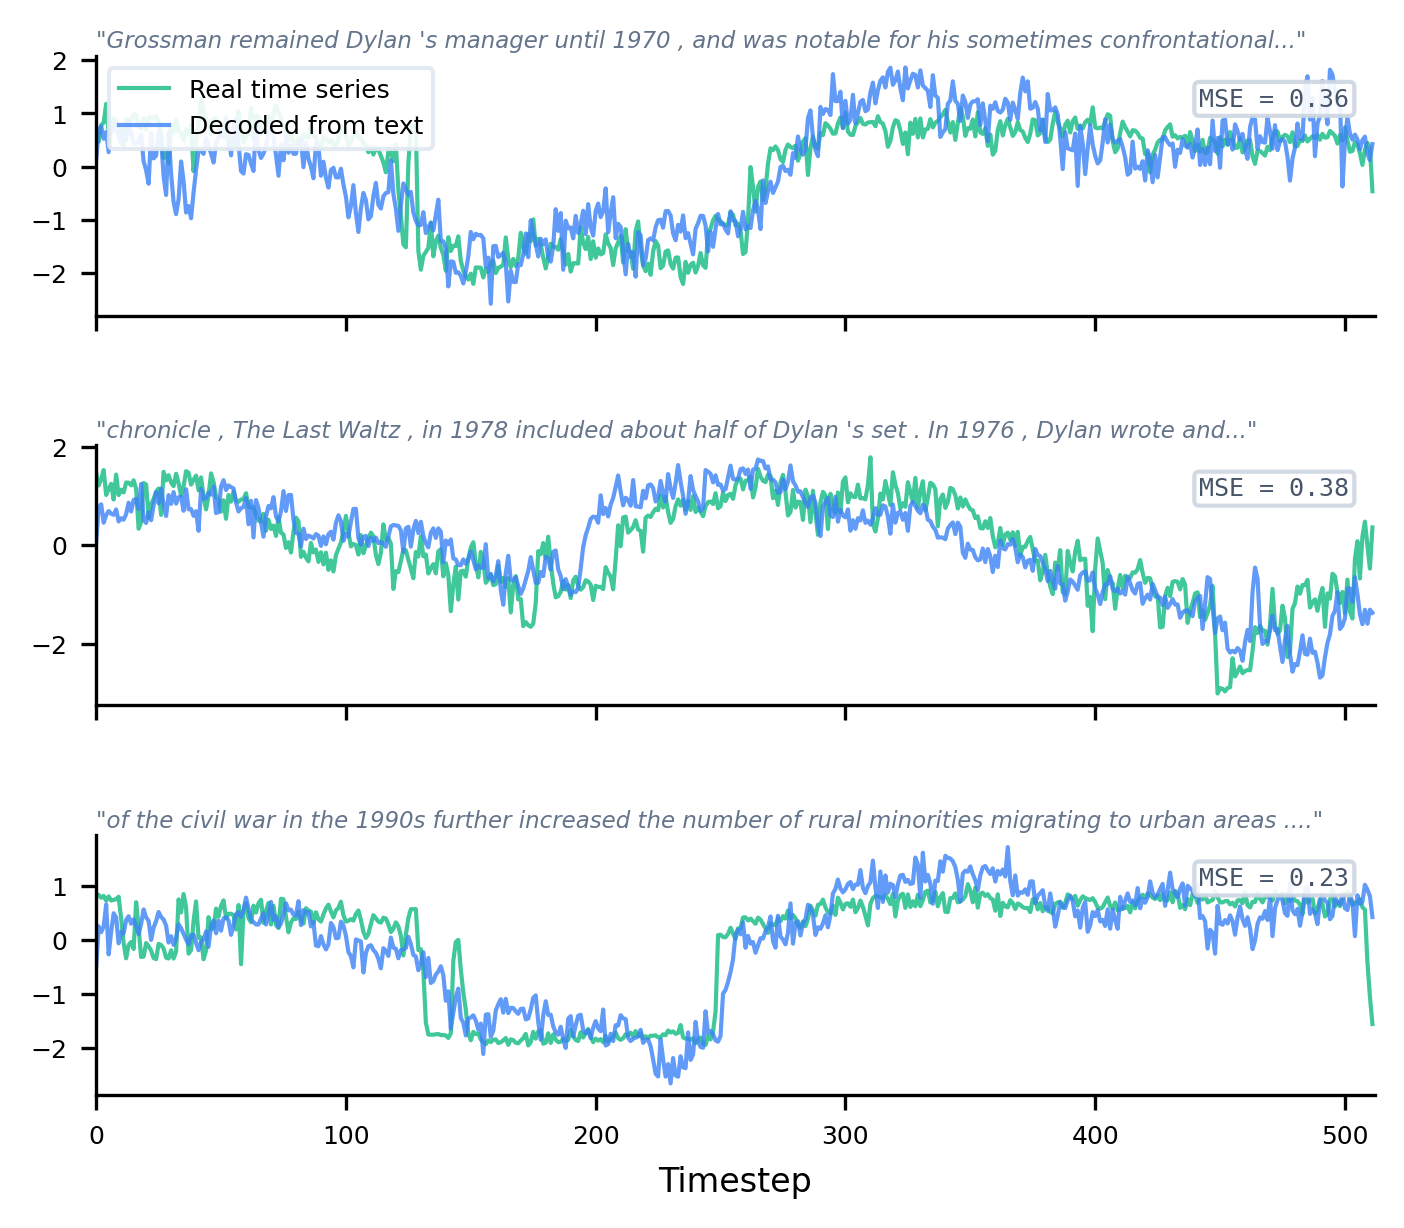
\includegraphics[width=\textwidth]{figures/sec4/panel_b_examples.png}
\caption{Decoded time series from text}
\label{fig:examples}
\end{subfigure}
\hfill
\begin{subfigure}[t]{0.48\textwidth}
\centering
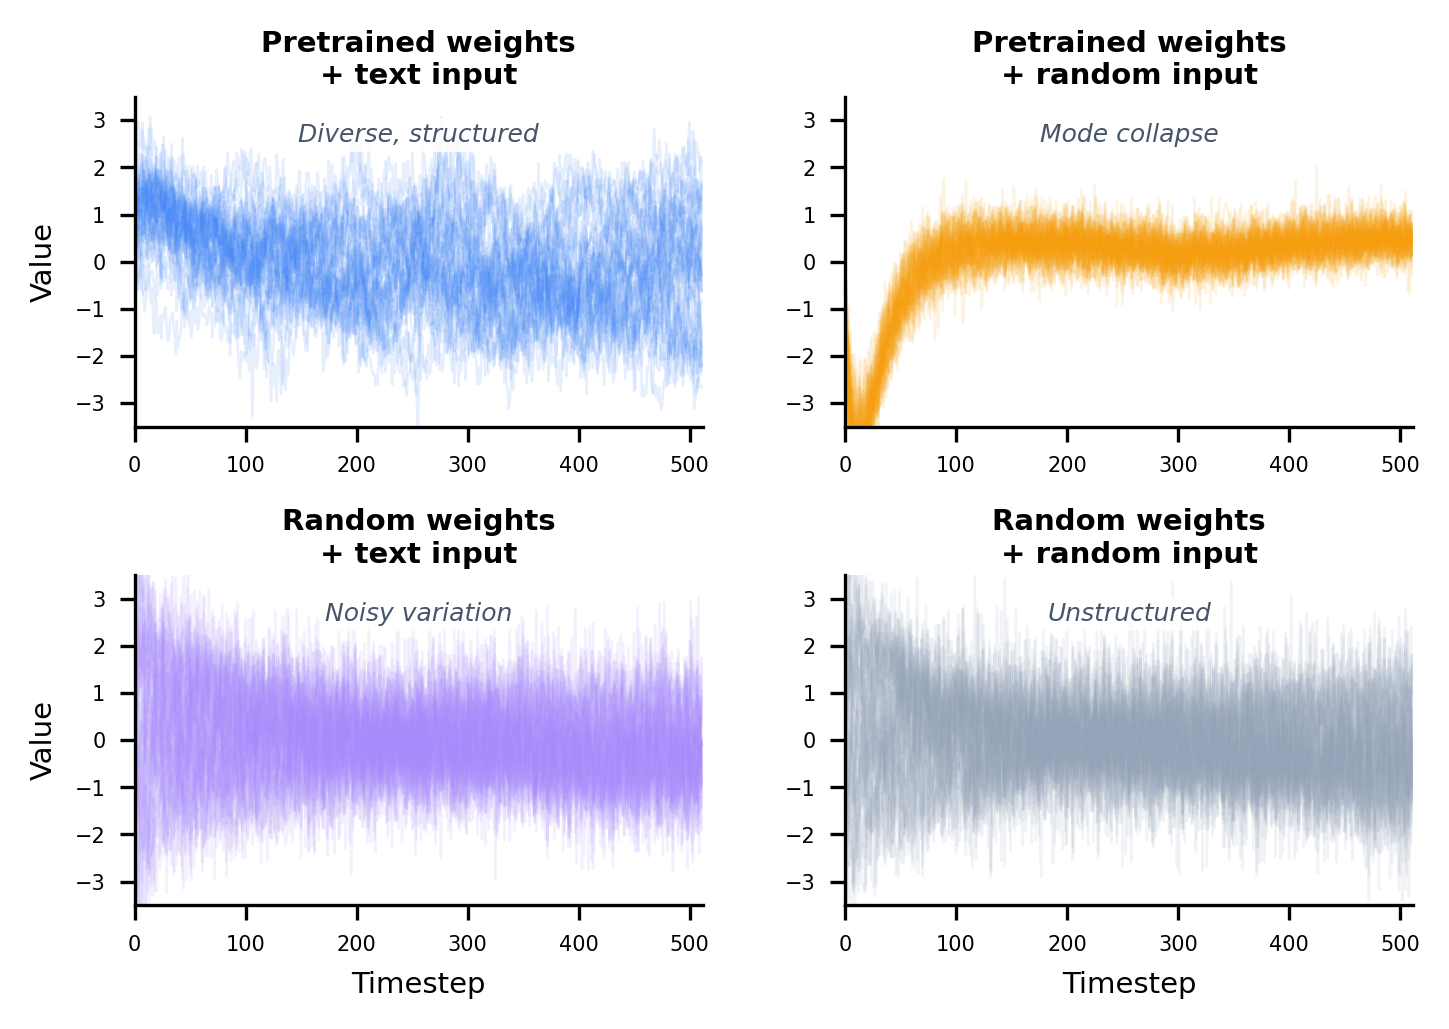
\includegraphics[width=\textwidth]{figures/sec4/panel_c_ablation.png}
\caption{Ablation: what creates the structure?}
\label{fig:ablation}
\end{subfigure}
\caption{\textbf{Pretrained hidden states contain time-series-compatible structure.} A single linear map $\hat{y}_t = \mathbf{w}^\top \mathbf{h}_t + b$ is trained on frozen LLM hidden states via EM-style nearest-neighbor matching to a bank of 10{,}000 real time series (no paired data). \textbf{(a)} Three decoded outputs (blue) overlaid with their nearest real time series (green). Input text shown above each plot. MSE $= 0.23$--$0.38$; full distribution in Appendix. \textbf{(b)} Ablation crossing learned weights vs.\ random init with text vs.\ random input. \emph{Top-left}: pretrained + text---diverse, structured outputs (301 unique matches). \emph{Top-right}: pretrained + random tokens---mode collapse to one shape (manifold exists but is not traversed). \emph{Bottom-left}: random weights + text---noisy variation without structure. \emph{Bottom-right}: random weights + random tokens---unstructured. Only pretrained weights \emph{and} meaningful text together produce diverse temporal signals.}
\label{fig:hero}
\end{figure}

\label{sec:linear_decoding}
 In these experiments, we learn an linear mapping, $\hat{y}_i \in \R^T$, provided in Eq.~\ref{eq:linear_map}, from a frozen, pre-trained language model's hidden states. For each WikiText sequence, hidden states are extracted from all 28 layers and concatenated per timestep, $\mathbf{h}_{i,t} = [\mathbf{h}_{i,t}^{(0)}; \ldots; \mathbf{h}_{i,t}^{(27)}] \in \R^{D}$, where $D$ is $28{,}672$. The per-timestep linear map then produces a predicted sequence that is z-normalized to zero mean and unit variance. Using an EM-style nearest-neighbor algorithm, each prediction is matched with its closest time series from GiftEval. Fig.~\ref{fig:ablation}(a) shows plots of three of these predictions (blue) along with their closest GiftEval matches (green), on a set of data not included in the training of the linear layer. The mapping is optimized to minimize MSE to these assignments, with a spectral diversity penalty, $\lambda$, to prevent collapse.
  \begin{equation}
 \label{eq:linear_map}
     \hat{y}_{i,t} = \mathbf{w}^\top \mathbf{h}_{i,t} + b
 \end{equation}
  
Out of $1920$ wiki text samples, the linear map produces $686$ unique matches to one of the $10{,}000$ real time series. The map generalizes to $439$ unique held-out WikiText text sequences out of $1000$, strongly suggesting that the pre-trained language model's representation space already contains directions whose projections resemble temporal signals.
 
The fact that linear probing can extract realistic time-series from language model hidden states has direct implications for fine-tuning these language models to predict time-series. Let $\mathcal{M} \subset \R^D$ denote the manifold of hidden-state trajectories produced by the pre-trained language model processing text. The experiments demonstrate the existence of a direction $\mathbf{w} \in \R^D$ such that the distribution of projected trajectories, $\{\mathbf{w}^\top \mathbf{h}_t\}_{t=1}^T$ has significant overlap with the distribution of real time series, $P_{\mathrm{TS}}$. If we define $\mathbf{h}*t$ as the hidden state of the pretrained model %at timestep $t$, 
due to its autoregressive training, the model implements a deterministic update shown in Eq.~\ref{eq:deterministic_update} and learns to predict $x_{t+1}$ from $\mathbf{h}_t$. In practice, this means that the model has learned structured dynamics over the hidden states and given $\mathbf{h}*t$, it can reliably produce the next state $\mathbf{h}*{t+1}$ along trajectories induced by natural text.

\begin{equation}
\label{eq:deterministic_update}
    \mathbf{h}_{t+1} = F(\mathbf{h}*t, x*{t+1})
\end{equation}

The linear probing experiments demonstrate that a projection direction, $\mathbf{w}$, resembling a real-world time series can indeed be found within the frozen language models representation space. Because the LLM is trained to predict the next token $x_{t+1}$ by evolving its internal state, the function $F$ in Eq.~\ref{eq:deterministic_update} acts as a latent dynamical system for the temporal manifold. The model must implicitly predict $\mathbf{h}_{t+1}$ to make autoregressive predictions so it already possess the ability to propagate these signals through time. Once obtained, $\mathbf{h}*{t+1}$ can be combined with the pre-existing direction $\mathbf{w}$ and applied to Eq.~\ref{eq:linear_map} to produce $y_{t+1} = \mathbf{w}^\top \mathbf{h}_{t+1}$. This confirms that the pre-trained language model ca propagate hidden states along trajectories consistent with real-world time series.

In summary, fine-tuning language models for time series does not require learning the dynamics from scratch, it is a low-dimensional alignment problem that requires selecting and scaling existing directions in representation space.

\subsection{this needs a new section or appendix relocation}
The latent temporal structure exhibited above could have a variety of explanations which we attempt to 
%transformer architectures possess residual connections that produce smooth trajectories, the learned weights (pretraining compresses representations), or the input (natural text has sequential structure). 
disentangle by crossing model weights (pretrained vs.\ randomly initialized, same architecture) with input (WikiText vs.\ random tokens). A clear interaction emerges, \textit{pre-trained weights} create a structured, low-dimensional manifold, but random tokens fail to traverse it, Tab.~\ref{tab:ablation} shows that \textit{rand+PT} collapses to just four unique outputs. \textit{Meaningful text} provides variation, but without pretrained weights, this variation is unstructured noise (Tab.~\ref{tab:ablation} \textit{text+RandInit}). Only the combination produces diverse, high-quality temporal signals. In this case, the pretrained manifold provides the geometry, and text input drives its diverse traversal.

\begin{table}[h]
\centering
\caption{$2\times 2$ ablation. \emph{Unique}: distinct real TS matched. \emph{NN}: mean nearest-neighbor MSE. Low NN with low Unique indicates mode collapse, not quality. We need to fix the NN because its not normalized by the number of matches}
\label{tab:ablation}
\begin{tabular}{lrrrr}
\toprule
Condition & Train Unique & Held-Out Unique & Held-Out NN & Clusters \\
\midrule
\textbf{text + PT}   & \textbf{686}/1920 & \textbf{439}/1000 & 0.717 & 14/20 \\
text + RandInit       & 54/1920           & 73/1000            & 0.541 & 13/20 \\
rand + PT             & 4/1920            & 1/1000             & 0.293 & 4/20  \\
rand + RandInit       & 99/1920           & 138/1000           & 0.741 & 14/20 \\
\bottomrule
\end{tabular}
\end{table}


\subsection{The Projected Dynamics Forecast Beyond the Context}
\label{sec:forecasting}

The linear decoding result shows shape-level similarity between projected hidden states and real time series. We test whether this extends to \emph{predictive} structure: given the first half of a time series, can a retrieved text projection forecast the second half?

\paragraph{Method.} We take 500 real time series from GiftEval and observe only the first 256 of 512 timesteps. Among 10{,}000 WikiText projections, we retrieve the one with lowest MSE on the observed first half and use that projections second half as the forecast. The baseline is last-value carry-forward \textit{i.e.} repeating the final observed value.

\paragraph{Result.} Across all 500 queries, the retrieval-based forecast achieves MSE $= 1.91$ versus last-values $2.27$ ($16\%$ lower). The retrieval wins in $37\%$ of cases; when it wins, the advantage is large (median $4\times$ lower MSE), because the retrieved projection captures trends and level shifts that last-value misses entirely. Figure~\ref{fig:forecasting} shows the best-case example from our evaluation set.

\begin{figure}[h]
\centering
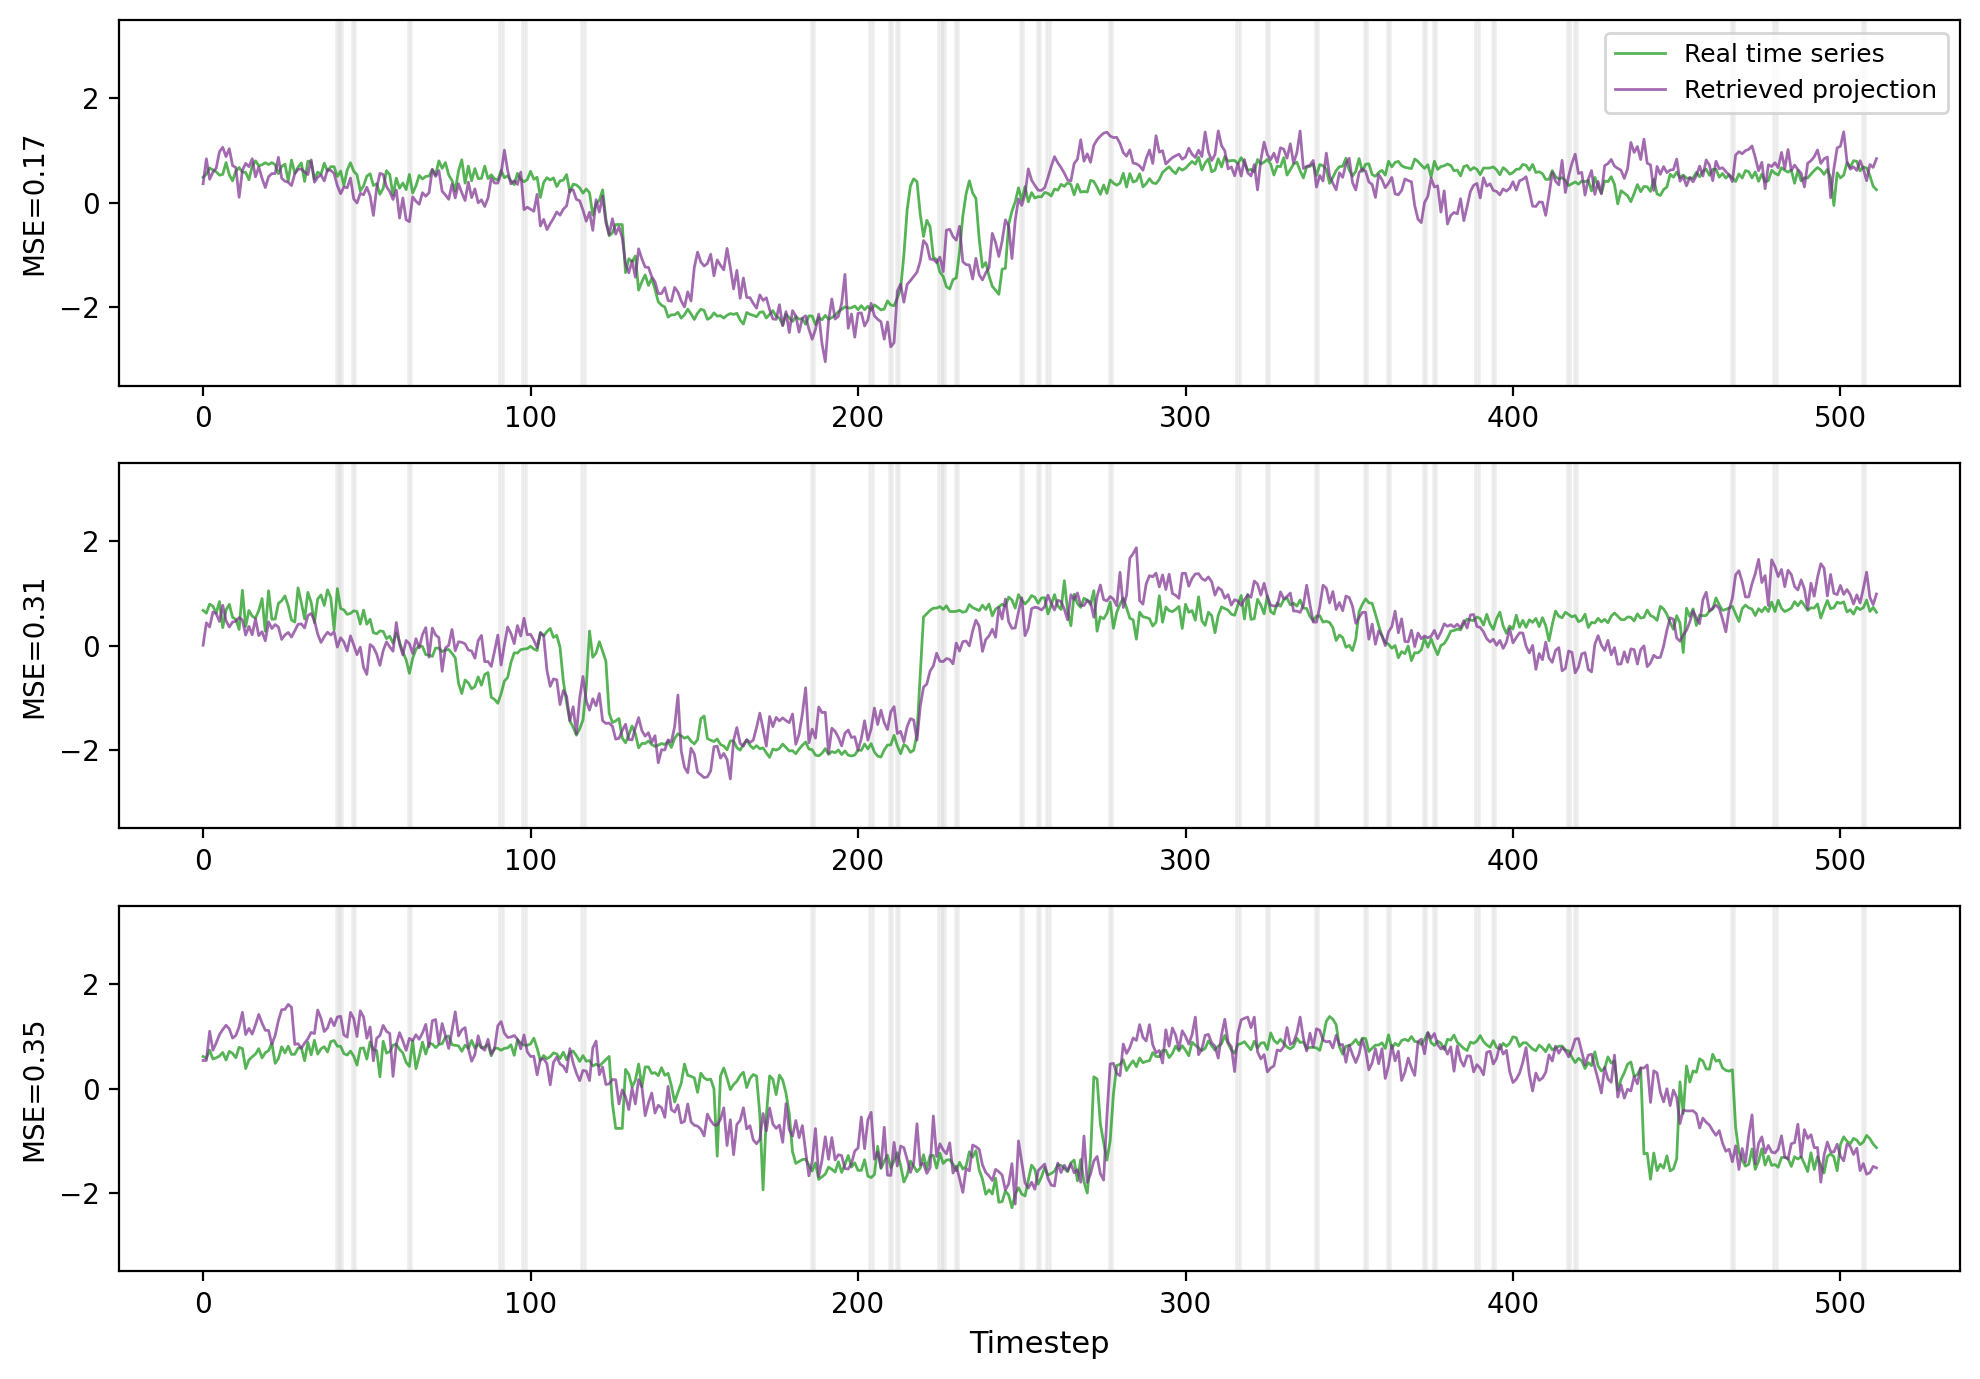
\includegraphics[width=\textwidth]{figures/sec4/panel_forecasting.png}
\caption{Forecasting example with largest gap compared to baseline from 500 evaluation queries. The first 256 timesteps are used to retrieve the closest WikiText projection; the projection's second half (purple) forecasts the continuation. The retrieved projection captures the level shift and subsequent trend (MSE $= 0.42$), while last-value carry-forward (gray dashed) is stranded at the final context value (MSE $= 11.7$).}
\label{fig:forecasting}
\end{figure}


\subsection{Pretraining Creates Coherent Gradient Signal for the TS Objective}
\label{sec:curvature}

\begin{figure}[h]
\centering
\includegraphics[width=\textwidth]{figures/sec4/fig_headline_7.png}
\caption{.}
\label{fig:grad_alignment}
\end{figure}

\textbf{details in the md file https://hackmd.io/VIS4nmT6Q2ms66mMUXTgWQ}

The manifold structure has direct consequences for optimization. We compute per-example gradients of the TS loss at the pretrained versus random initialization, measuring whether individual training examples provide coherent or contradictory optimization signals.

\paragraph{Method.} For 30 individual TS sequences, we compute the gradient $\mathbf{g}_i = \nabla_\theta L_i$ restricted to layers 6--10 (78.7M parameters) at both initializations. We measure pairwise cosine similarity $\cos(\mathbf{g}_i, \mathbf{g}_j)$ across all example pairs, and the signal-to-noise ratio $\mathrm{SNR} = \|\bar{\mathbf{g}}\| / \mathrm{mean}(\|\mathbf{g}_i - \bar{\mathbf{g}}\|)$.

\begin{table}[h]
\centering
\caption{Per-example gradient structure at the TS loss surface. At PT initialization, different TS examples produce gradients that reinforce each other. At random initialization, gradients are nearly orthogonal and cancel upon averaging.}
\label{tab:gradient_alignment}
\small
\begin{tabular}{lcc}
\toprule
Metric & PT init & Random init \\
\midrule
Per-example gradient cosine & \textbf{0.58} & 0.04 \\
Gradient signal-to-noise ratio & \textbf{1.16} & 0.28 \\
Gradient norm (RMS) & 0.0040 & 0.0004 \\
\bottomrule
\end{tabular}
\end{table}

\paragraph{Interpretation.} At PT initialization, per-example TS gradients have cosine similarity 0.58---different time series sequences agree on which direction to adjust the weights. Batch averaging reinforces this shared signal. At random initialization, gradients are nearly orthogonal (cosine 0.04, consistent with random vectors in $\sim$78M dimensions), so averaging causes massive cancellation: the SNR drops to 0.28, meaning most of the per-example gradient signal is lost.

This coherence arises because the pretrained representations create consistent feature activations across different TS inputs. When the loss asks ``how should this weight change?'', the answer is similar regardless of which TS sequence is used, because the pretrained features impose a shared structure on the loss landscape. At random initialization, each example activates arbitrary features, giving contradictory signals.

The effect is layer-dependent: gradient norms at PT initialization are 3--19$\times$ larger than at random initialization, with the ratio increasing for deeper layers (where random weights scramble the signal most). This layer-wise gradient structure explains why mid-to-deep layers benefit most from pretrained initialization (Section~\ref{sec:dimensionality}).

% Rerun this and the above across multiple checkpoints
\paragraph{Curvature anisotropy.} To characterize the \emph{shape} of the loss landscape, we compute the curvature $\mathbf{v}^\top H \mathbf{v}$ along 200 random unit vectors $\mathbf{v}$ in layers 6--10 parameter space using exact Hessian-vector products (Pearlmutter trick), and compare this to the curvature along the gradient direction $\hat{\mathbf{g}}$. At PT initialization, the gradient direction has curvature $232$, while the mean curvature across random directions is $9.6 \times 10^{-5}$---a ratio of $2.4 \times 10^6$. At random initialization, the gradient direction has curvature $-0.08$ (near-zero, slightly negative), barely distinguishable from random directions (mean $8.4 \times 10^{-7}$, ratio $\sim$80$\times$). The PT landscape is thus \emph{massively anisotropic}: SGD's natural descent direction is aligned with one of the very few high-curvature directions in a $\sim$78M-dimensional space, while the vast majority of directions are flat. At random initialization, the landscape is nearly isotropic---all directions, including the gradient, have negligible curvature.
% ═══════════════════════════════════════════════════════════════


% ═══════════════════════════════════════════════════════════════
\section{Finetuning Projects the Pretrained Manifold onto Time Series}
\label{sec:finetuning}


\subsection{The Weight Changes are Low-Rank}
\label{sec:lora}

% LoRA vs IO-only vs full finetuning comparison
% Key point: LoRA with small rank captures most of the transfer benefit,
% proving only a low-rank perturbation of the weights is needed.

% ── TABLE: Finetuning regime comparison ──
\begin{table}[h]
\centering
\caption{Finetuning regime comparison on GiftEval ND[0.5]. TODO: fill from Alexis's experiments.}
\label{tab:lora}
\begin{tabular}{lccc}
\toprule
Method & Params changed & ND[0.5] & \% of full FT \\
\midrule
Full finetuning     & 100\%  & TODO & 100\%  \\
LoRA ($r=16$)       & TODO\% & TODO & TODO\% \\
LoRA ($r=4$)        & TODO\% & TODO & TODO\% \\
IO-only (emb + head)& TODO\% & TODO & TODO\% \\
Random init (full)  & 100\%  & TODO & ---    \\
\bottomrule
\end{tabular}
\end{table}

\paragraph{Interpretation.} Only a low-rank perturbation of the pretrained weights is needed to adapt the model from language to time series. This means the bulk of the pretrained computation is preserved---finetuning adjusts a small subspace of directions.


\subsection{Finetuning Selects Useful Directions}
\label{sec:dimensionality}

% Table moved to appendix (Table~\ref{tab:effrank} and Table~\ref{tab:alignment})

% ── FIGURE: Effective rank + Subspace alignment across layers ──
\begin{figure}[!ht]
\centering
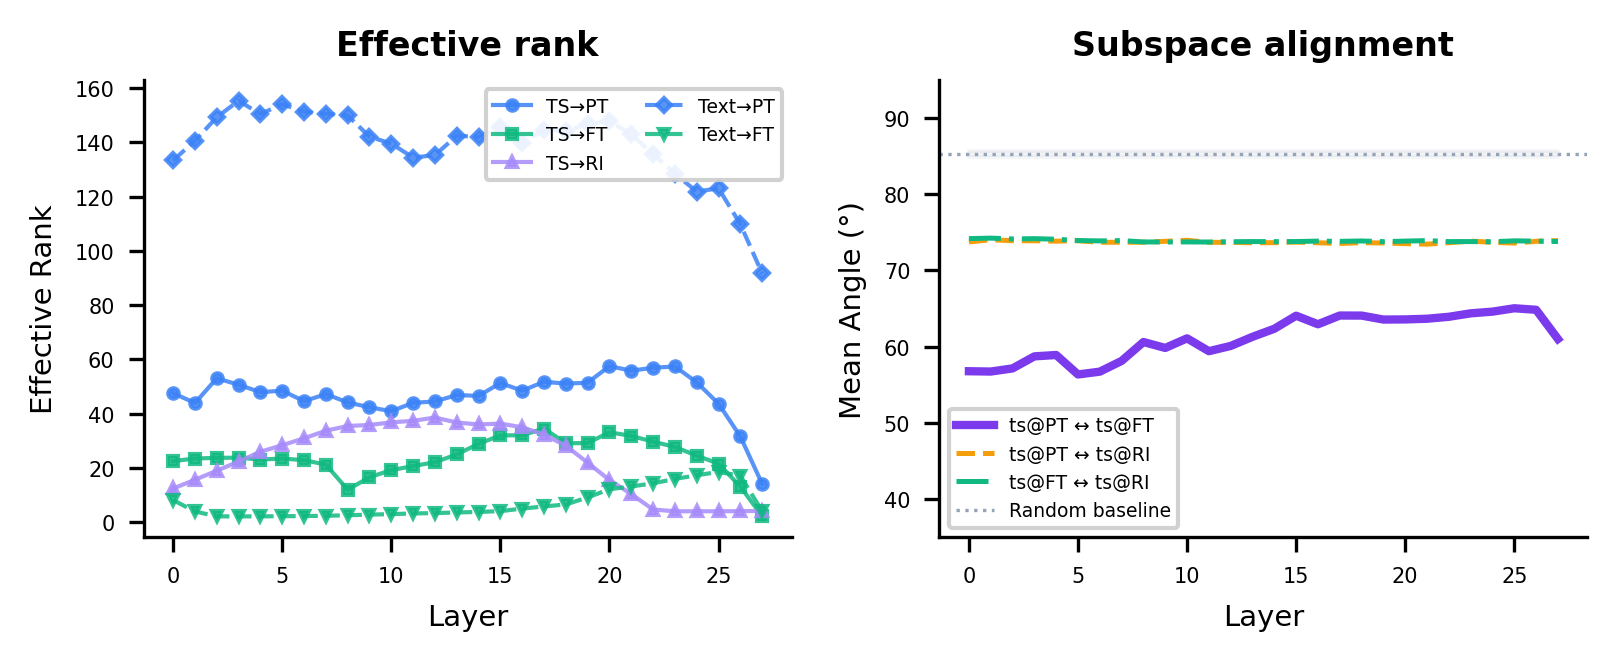
\includegraphics[width=0.95\textwidth]{figures/sec5/fig_geometry.png}
\caption{\textbf{Geometric evidence for direction reuse.} \textbf{(Left)} Effective rank across layers. FT compresses TS representations to $\sim$12 dimensions (green solid), far below PT's $\sim$44 (blue solid) and RI's $\sim$35 (purple solid). Text$\to$FT collapses to $\sim$2.5 (catastrophic forgetting). \textbf{(Right)} Subspace alignment: mean principal angle between top-10 PCs. ts@PT$\leftrightarrow$ts@FT (purple) stays well below the random baseline (85.3$^\circ$), confirming FT reuses PT's directions. Tables~\ref{tab:effrank} and~\ref{tab:alignment} in Appendix.}
\label{fig:geometry}
\end{figure}

\paragraph{Catastrophic forgetting as geometric compression.}
Text$\to$FT collapses to effective rank 2.5 (from 150 in PT). Finetuning traded $\sim$140 text-useful dimensions for $\sim$12 TS-useful dimensions.

\paragraph{Method: effective rank across training.}
To track how representational geometry evolves during training, we compute the effective rank of hidden-state covariance matrices at every saved checkpoint. For each checkpoint and each of the 28 transformer layers, we pass 10{,}000 time-series windows (length 512, drawn from the GiftEval validation split) through the model, collecting hidden states at every position except position~0 (excluded to avoid the attention-sink artifact). For FT and FT\textsubscript{IO} we additionally pass 10{,}000 WikiText-103 sequences to track text representation quality.

At each layer we accumulate the centered covariance matrix $\Sigma = \frac{1}{N}\sum_i \mathbf{h}_i \mathbf{h}_i^\top - \bar{\mathbf{h}}\bar{\mathbf{h}}^\top$ in float64 over all $N$ hidden-state vectors ($N \approx 130{,}000$ per batch), then compute its eigendecomposition. The effective rank is $\mathrm{erank}(\Sigma) = \exp\!\bigl(-\sum_i p_i \log p_i\bigr)$, where $p_i = \lambda_i / \sum_j \lambda_j$ are the normalized eigenvalues~\citep{roy2007effective}. This equals 1 when all variance concentrates on a single direction and equals the ambient dimension $d$ when variance is uniformly spread.

We evaluate all checkpoints for three training regimes: FT (full finetuning from PT, 15 checkpoints from step 1 to 10{,}000), FT\textsubscript{IO} (input/output layers only, 17 checkpoints from step 1 to 33{,}000), and RI (randomly initialized, 14 checkpoints from step 1 to 8{,}192). The pretrained model (PT) serves as a fixed baseline. Checkpoints are processed 4 at a time across 4 GPUs.

\begin{figure}[!ht]
\centering
\begin{subfigure}[t]{0.48\textwidth}
\centering
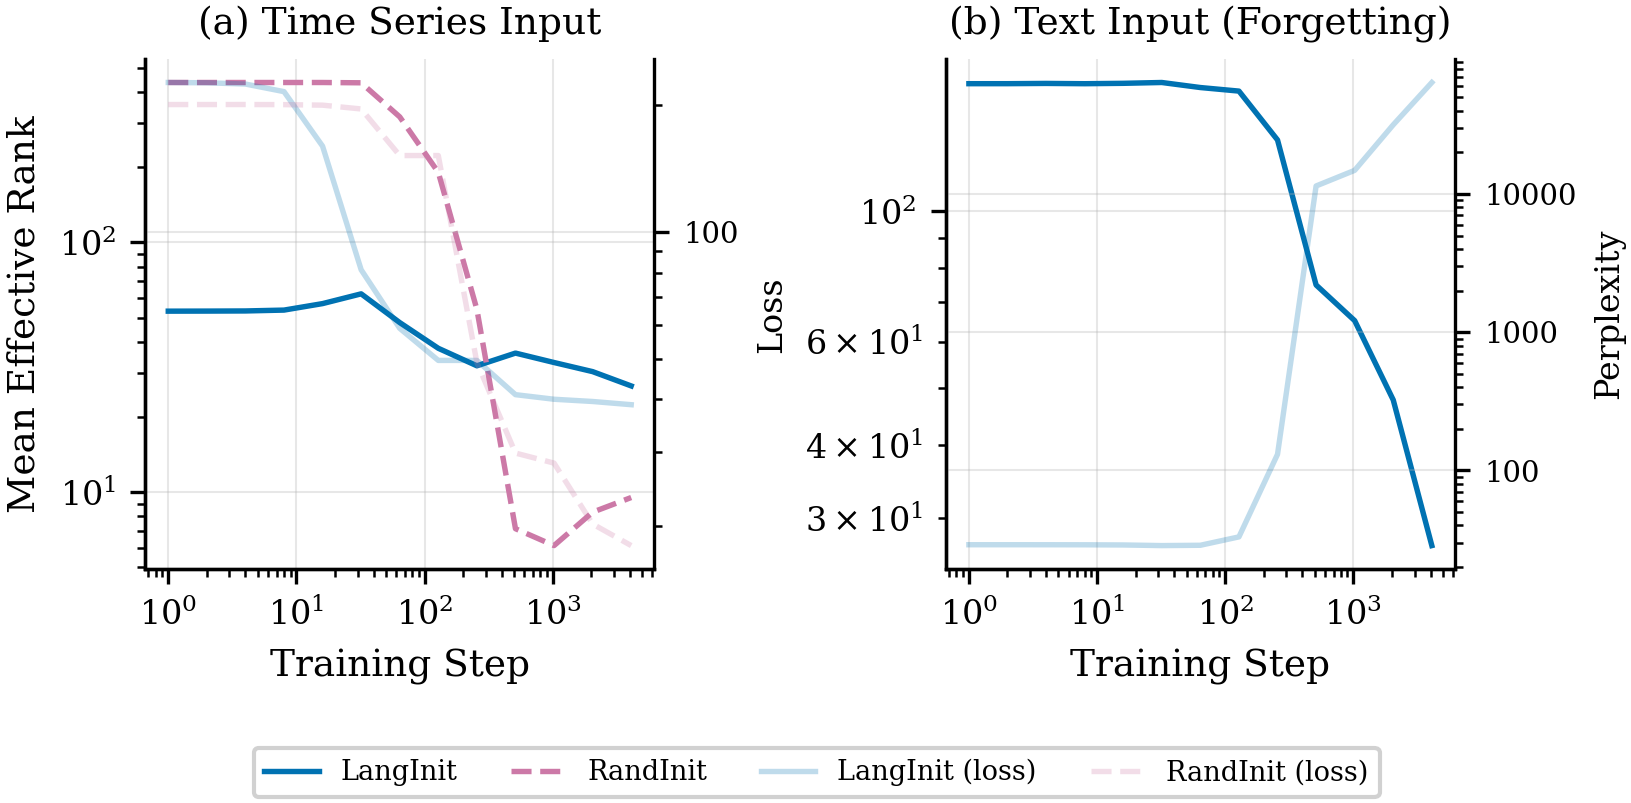
\includegraphics[width=\textwidth]{figures/sec5/fig_erank_trajectory.png}
\label{fig:erank_trajectory}
\end{subfigure}
\hfill
\begin{subfigure}[t]{0.48\textwidth}
\centering
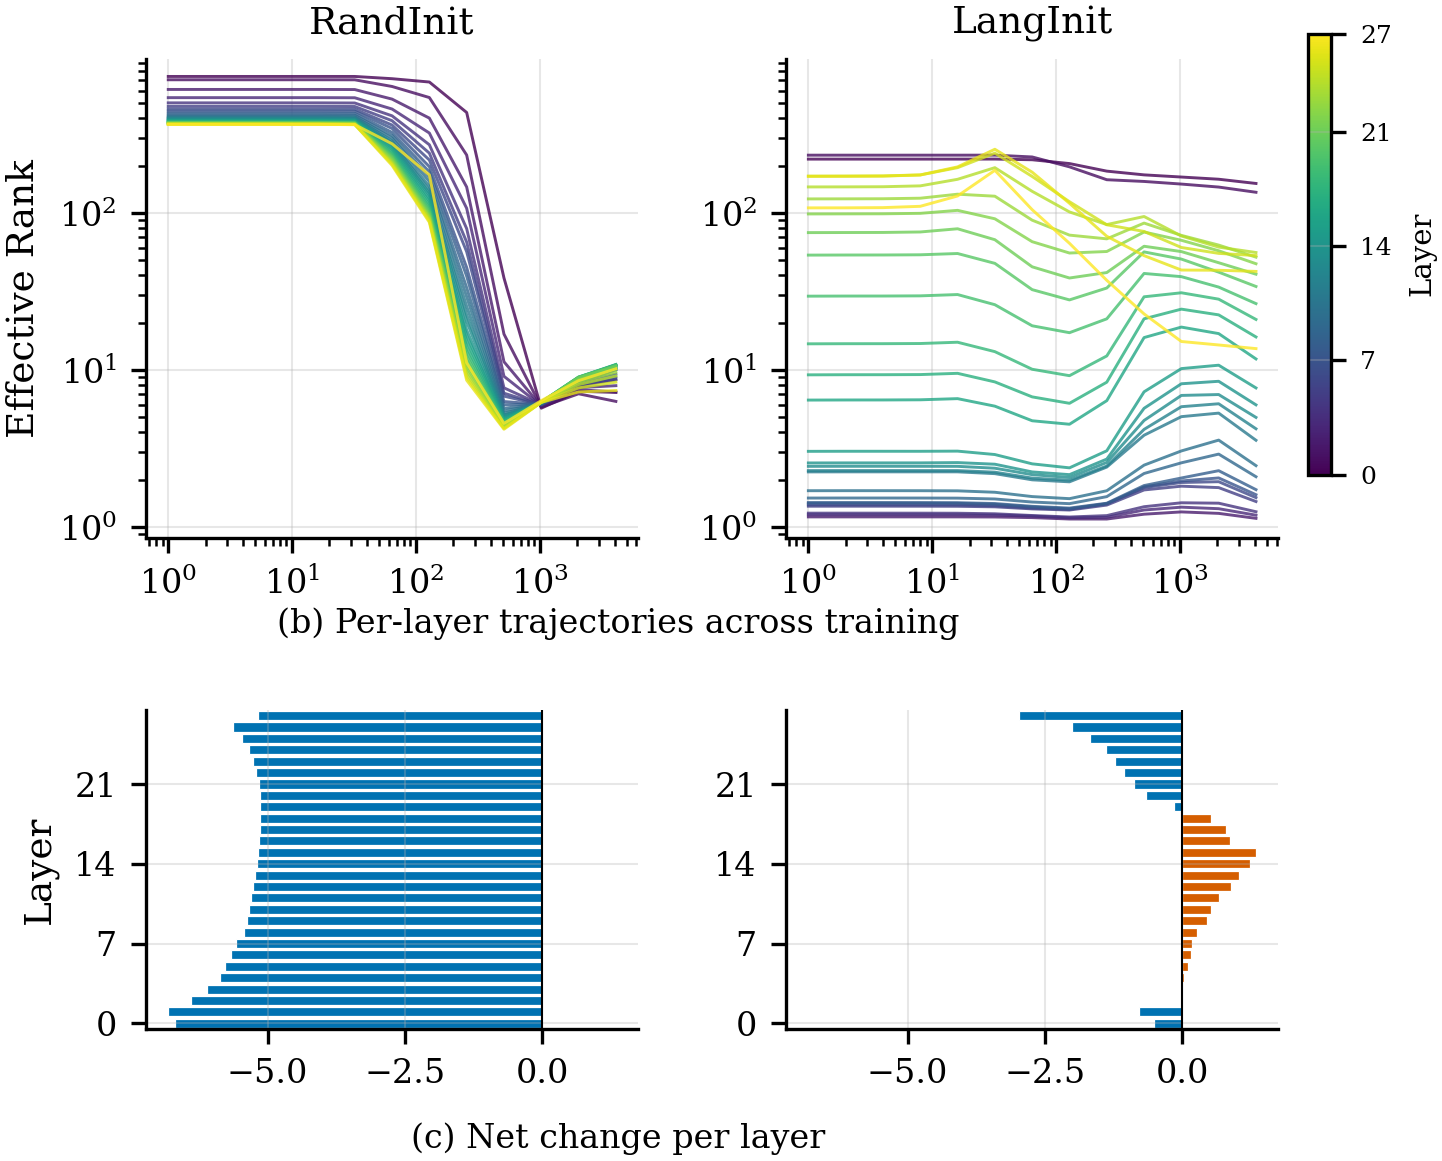
\includegraphics[width=\textwidth]{figures/sec5/fig_erank_layers.png}
\label{fig:erank_layers}
\end{subfigure}
\caption{\textbf{Effective rank dynamics during training.} \textbf{(a)}~Mean effective rank across all 28 layers. Left: on time-series input, RandInit starts near-isotropic ($\sim$440) and collapses to $\sim$10 within 500 steps; LangInit declines more gradually from the pretrained baseline ($\sim$50) to $\sim$27. Transparent lines show CRPS loss on a secondary axis. Right: on text input, LangInit's effective rank drops from $\sim$165 to $\sim$25 (85\% reduction) while perplexity rises, confirming catastrophic forgetting. \textbf{(b)}~Per-layer trajectories (each line = one of 28 layers, colored by depth). RandInit layers collapse as a tight bundle; LangInit middle layers ($\sim$8--17) \emph{increase} their effective rank while early and late layers decrease. \textbf{(c)}~$\log_2$ change (final/initial) per layer. Orange = gained rank; blue = lost. RandInit is uniformly negative ($-5$ to $-7$, i.e., 32--128$\times$ reduction). LangInit layers 10--17 show positive change (up to $+1$ log$_2$ = $2\times$ increase)---finetuning redistributes capacity from the network's periphery to its core.}
\label{fig:erank_dynamics}
\end{figure}


\subsection{Reuse vs.\ Reinvention: LangInit and RandInit Find Different Solutions}
\label{sec:reuse_vs_reinvent}

\paragraph{Method.}
To probe how each model geometrically encodes temporal structure, we pass synthetic waveforms through the network and visualize hidden-state trajectories via 2D PCA. We generate five inputs of length 512: a sine wave (period~64), a square wave (period~64), a sawtooth wave (period~64), a two-frequency signal ($\sin(2\pi t/64) + 0.5\sin(2\pi t/17)$), and a linear trend with oscillation ($t/T + 0.3\sin(2\pi t/80)$). Each input is independently $z$-score normalized, clipped to $[-5, 5]$, and uniformly binned into 1024 tokens. The tokenized sequence is passed through the model, and we extract hidden states at the target layer. PCA is fitted independently per model--input pair, since the models occupy different regions of representation space. The first 5 positions are excluded to avoid the attention-sink artifact. Trajectories are colored by input phase (position mod period / period) to reveal periodic structure. Full per-layer breakdowns for all 28 layers are provided in Figures~\ref{fig:pca_grid_ft} and~\ref{fig:pca_grid_ri} in the Appendix.

% ── FIGURE: Sine layer evolution + coherence evolution ──
\begin{figure}[!ht]
\centering
\begin{minipage}[t]{0.42\textwidth}
\centering
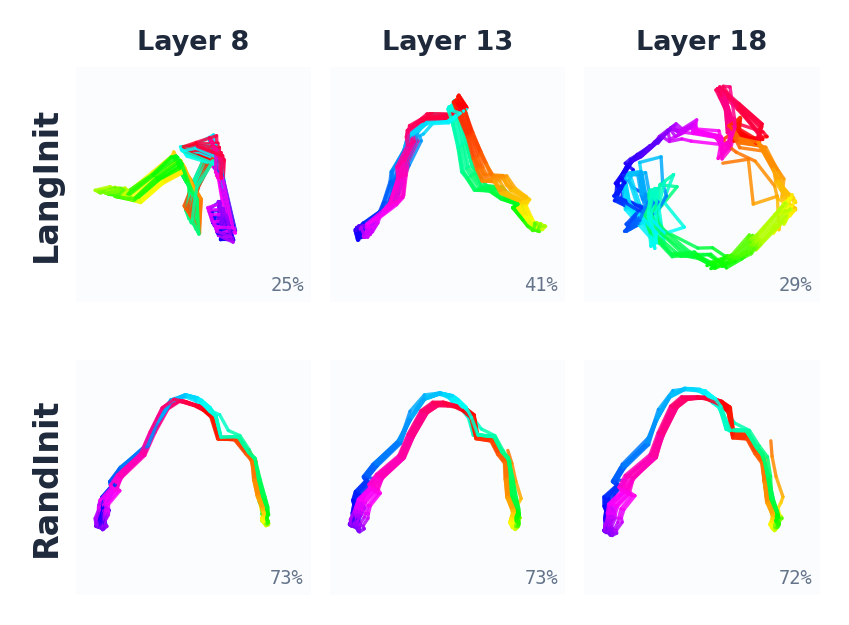
\includegraphics[width=\textwidth]{figures/sec5/fig_sine_evolution.png}
\end{minipage}%
\hfill
\begin{minipage}[t]{0.56\textwidth}
\centering
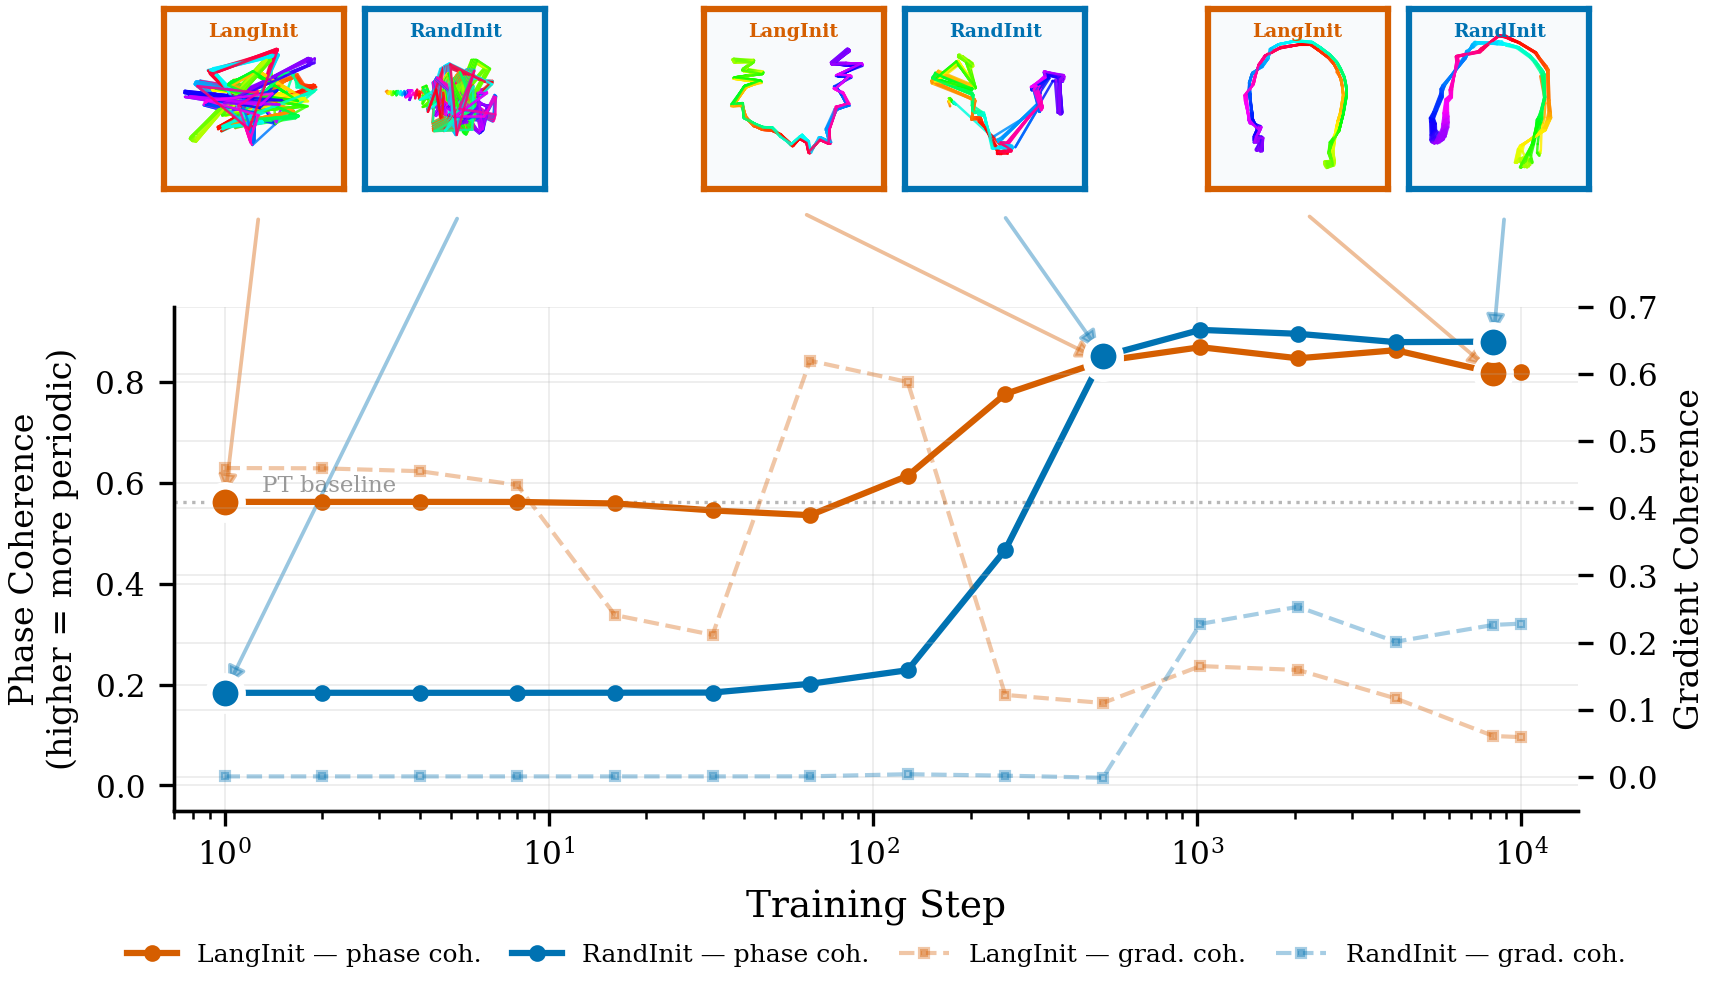
\includegraphics[width=\textwidth]{figures/sec5/fig_coherence_evolution.png}
\end{minipage}
\caption{\textbf{Left: Sine wave representations across layers.} A sine wave (period~64) passed through LangInit (top) and RandInit (bottom) at layers 8, 13, and 18, shown as 2D PCA colored by input phase. RandInit produces clean arcs at every layer (72--73\% PCA variance); LangInit produces complex, layer-varying loops (25--41\%).
\textbf{Right: Phase and gradient coherence across training.} Phase coherence (solid; $1 - \text{same-phase} / \text{all-pair distance ratio}$, higher = more periodic) and gradient coherence (dashed) at Layer~13. Insets show t-SNE of hidden states at steps 1, 512, and 8192. LangInit inherits periodic structure from pretraining and starts high; RandInit starts near zero and undergoes an abrupt phase transition around step~256--512 where gradient coherence simultaneously spikes, indicating that the model discovers periodic geometry at the same moment it begins aligning gradients across the time series.}
\label{fig:sine_evolution}
\end{figure}

Figure~\ref{fig:sine_evolution} (left) shows this contrast for a single sine wave across three representative layers. RandInit converges to a uniform, clean arc at every layer, with 72--73\% of variance explained by just two principal components. LangInit produces complex, layer-specific loops with only 25--41\% PCA variance---the periodic structure is distributed across many more dimensions, reflecting the richer geometry inherited from pretraining. Figure~\ref{fig:sine_evolution} (right) tracks how this geometry emerges during training: LangInit inherits high phase coherence from the start, while RandInit undergoes a sharp phase transition around step~256--512 that coincides with a spike in gradient coherence.

% ── FIGURE: Synthetic inputs PCA at Layer 13 ──
\begin{figure}[!ht]
\centering
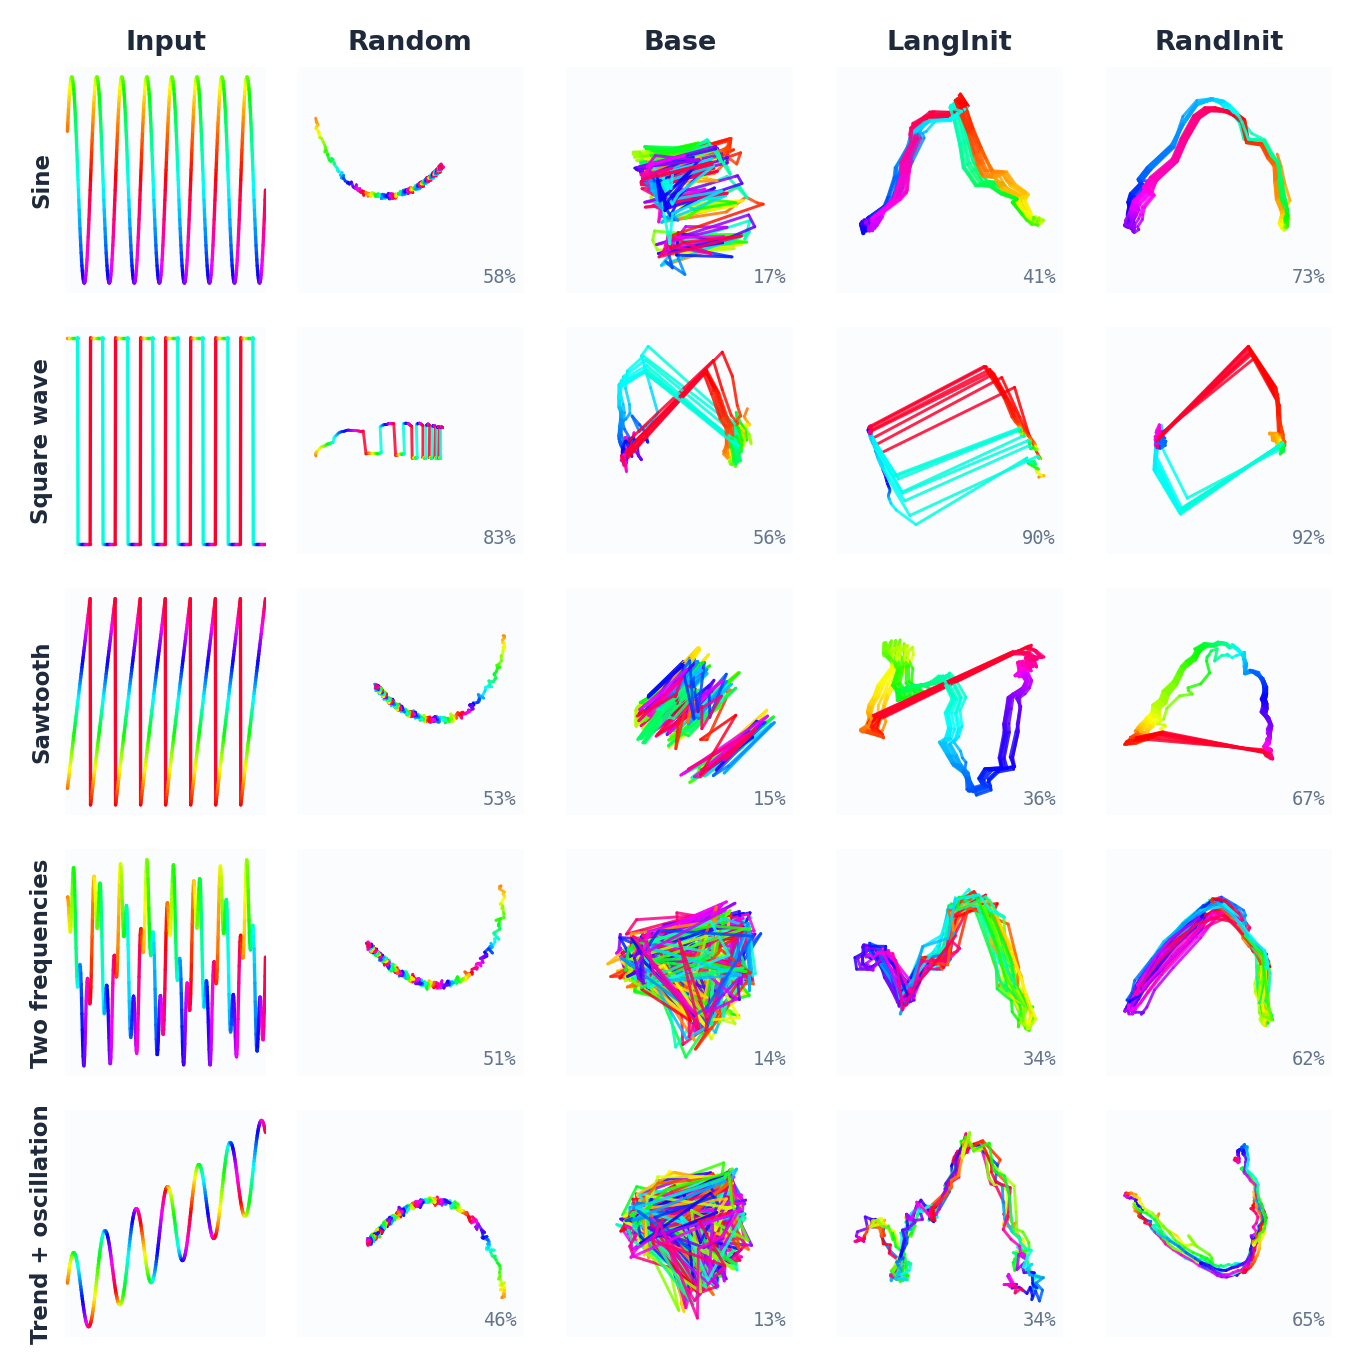
\includegraphics[width=0.85\textwidth]{figures/sec5/fig_synthetic_L13_pca.png}
\caption{\textbf{Hidden-state trajectories for synthetic inputs at Layer~13 (PCA).} Each row is a different input waveform; columns show a randomly initialized untrained model (Random), the pretrained LLM (Base), the language-initialized model finetuned on time series (LangInit), and the randomly-initialized model trained on time series (RandInit). Trajectories are 2D PCA projections of hidden states, colored by input phase. Percentages show variance captured by 2 PCs. Random and Base produce unstructured trajectories. RandInit discovers clean, low-dimensional representations (62--92\% PCA variance) while LangInit creates geometrically complex but structured trajectories (34--98\%) that vary by input type.}
\label{fig:synthetic_pca}
\end{figure}

Figure~\ref{fig:synthetic_pca} extends this analysis to all five synthetic inputs at Layer~13. RandInit consistently produces clean, geometrically simple trajectories with high PCA variance, while LangInit creates more complex structures that vary by input type. Notably, both models arrive at representations that capture the same underlying temporal patterns---the t-SNE projections in Figure~\ref{fig:synthetic_tsne} (Appendix) confirm that the global geometries arrive at the same solution. The key difference is \emph{interpretability}: RandInit's representations are more readily decomposed by linear methods (PCA), whereas LangInit distributes information nonlinearly across more dimensions. The training dynamics of these representations are visualized in Figures~\ref{fig:evolution_grid_ft} and~\ref{fig:evolution_grid_ri} in the Appendix and confirm that pretrained models reuse the complex, high effective rank solutions confirmed in Figure~\ref{fig:erank_dynamics}, while RandInit first simplifies the geometry before increasing complexity (and associatively effective rank) and converging to a solution.

\subsection{Interpreting the Transferred Features}
\label{sec:crosscoder_features}

\paragraph{Method.}
We train one sparse crosscoder per layer with a shared encoder and separate PT/FT decoders. The encoder maps pretrained-model activations on decimal-string time series and finetuned-model activations on binned time series into a shared 4{,}096-dimensional Top-$K$ latent space; PT--FT features are ranked by cross-domain firing balance and probed on WikiText-103.

\begin{table}[h]
\centering
\small
\caption{Examples of shared PT--FT crosscoder features. Shared features concentrate in layers~7--10; the examples below link concrete time-series motifs to coherent WikiText genres. Full examples are in Appendix~\ref{app:crosscoder}.}
\label{tab:crosscoder_features_main}
\begin{tabularx}{\linewidth}{clXX}
\toprule
Layer & Feature & Time-series motif & WikiText motif \\
\midrule
10 & 1712 & magnitude jumps / plateaus & measurements and unit conversions \\
9  & 2469 & volatile regime changes & tropical cyclone narratives \\
7  & 3888 & isolated spikes & timestamped naval battles \\
8  & 2567 & missing / NaN windows & \texttt{<unk>} and incomplete references \\
\bottomrule
\end{tabularx}
\end{table}

Thus, the aligned LangInit subspace is populated by reusable primitives, not just arbitrary low-rank directions. In Appendix~\ref{app:circuit}, we present a preliminary causal circuit analysis that provides additional evidence: zero-ablation identifies a superadditive circuit in Layer~1 (head~L1H4 $\leftrightarrow$ MLP\textsubscript{L1}) that is critical for periodic time-series prediction in FT\textsubscript{IO} and, in the pretrained model, is most important for text with sequential repetitive structure.
% ═══════════════════════════════════════════════════════════════

% ═══════════════════════════════════════════════════════════════
\section{Discussion and Limitations}
\label{sec:discussion}

\paragraph{The full picture.}
% Autoregressive pretraining creates smooth, low-dimensional trajectories (Section 3).
% This manifold contains directions naturally compatible with temporal data.
% Finetuning identifies the useful directions and compresses to them (Section 4.2),
% reusing pretrained structure rather than learning from scratch (Section 4.3).
% The transferred features are structural primitives—repetition, slopes, periodicity (Section 4.4).

\paragraph{Implications.}
% - Transfer should work for any pretrained autoregressive model, not just LLMs
% - The key property is smooth, low-dimensional sequential representations
% - The scaling result (pretrained 0.6B ≈ random 4B) suggests transfer provides
%   an ~8× effective parameter multiplier
% - LoRA's success suggests principled ways to preserve more pretrained structure

\paragraph{Limitations.}
% - Single architecture family (Qwen3), though multiple scales
% - GiftEval benchmark (diverse but finite)
% - Crosscoder dead features (40-60% per layer), limiting feature-level conclusions
% - The geometric analysis is descriptive—we characterize what changes but
%   cannot fully explain why specific directions are useful
% - Circuit analysis was inconclusive on the exact text computation being repurposed


\section{Conclusion}
\label{sec:conclusion}

% Language-to-TS transfer works because pretraining creates a geometric prior:
% a low-dimensional, smooth, anisotropic representation space.
% Finetuning projects this manifold onto time series by selecting the subset
% of pretrained directions useful for temporal data.
% The transferred features are structural primitives shared between language
% and time series—repetition, slopes, periodicity.
% The connection is geometric and structural, not semantic.

% ═══════════════════════════════════════════════════════════════


% \section*{References}
\small
\bibliographystyle{plainnat}
\bibliography{references}
% References follow the acknowledgments in the camera-ready paper. Use unnumbered first-level heading for
% the references. Any choice of citation style is acceptable as long as you are
% consistent. It is permissible to reduce the font size to \verb+small+ (9 point)
% when listing the references.
% Note that the Reference section does not count towards the page limit.

%%%%%%%%%%%%%%%%%%%%%%%%%%%%%%%%%%%%%%%%%%%%%%%%%%%%%%%%%%%%

\newpage
\appendix

\section{Additional Tables}

\begin{table}[h]
\centering
\caption{Representational geometry at Layer 8 for three models processing the same TS input.}
\label{tab:effrank}
\begin{tabular}{lrrrrr}
\toprule
Condition & Eff.\ Rank & PCs for 90\% & Speed & Low Freq \% \\
\midrule
TS $\to$ PT  & 44 $\pm$ 29  & 63  & 16  & 34.5\% \\
TS $\to$ FT  & \textbf{12 $\pm$ 6}  & \textbf{15}  & 64  & \textbf{52.3\%} \\
TS $\to$ RI  & 35 $\pm$ 21  & 46  & 78  & 44.7\% \\
\midrule
Text $\to$ PT & 150 $\pm$ 8  & 166 & 24  & 21.4\% \\
Text $\to$ FT & 2.5 $\pm$ 1.5 & 3  & 355 & 16.4\% \\
\bottomrule
\end{tabular}
\end{table}

\begin{table}[h]
\centering
\caption{Mean principal angle between top-10 PCs of each condition pair at Layer 8. Random baseline: 85.3$^\circ$ $\pm$ 0.4$^\circ$.}
\label{tab:alignment}
\begin{tabular}{lrl}
\toprule
Pair & Mean Angle & Significance \\
\midrule
\textbf{ts@PT vs ts@FT} & \textbf{60.6$^\circ$} & most aligned \\
ts@PT vs ts@RI           & 73.7$^\circ$ & aligned but less \\
ts@FT vs ts@RI           & 73.7$^\circ$ & --- \\
text@PT vs text@FT       & 79.9$^\circ$ & partially shifted \\
text@PT vs text@RI       & 85.4$^\circ$ & $\approx$ random \\
\bottomrule
\end{tabular}
\end{table}

\begin{table}[h]
\centering
\caption{Top cross-domain features (PT\_FT). Each fires on specific text patterns \emph{and} time series patterns.}
\label{tab:features_appendix}
\begin{tabular}{clp{4.5cm}p{4.5cm}}
\toprule
Layer & Name & Text activation & TS activation \\
\midrule
8  & Repetition detector  & ``$3 \cdot 3 \cdot 3 \cdot 3$'', ``2--3--2 config'' & Square waves, periodic oscillations \\
26 & Slope detector       & ``derivative'', ``tangent line'' & Rising/falling slopes \\
4  & Metronome detector   & ``tempo'', ``beats'' & Sharp periodic spikes \\
5  & Chord detector       & ``F--E$\flat$--G'' progressions & Periodic peaks \\
\bottomrule
\end{tabular}
\end{table}

\section{Reuse vs.\ Reinvention: Additional Figures}

\begin{figure}[!ht]
\centering
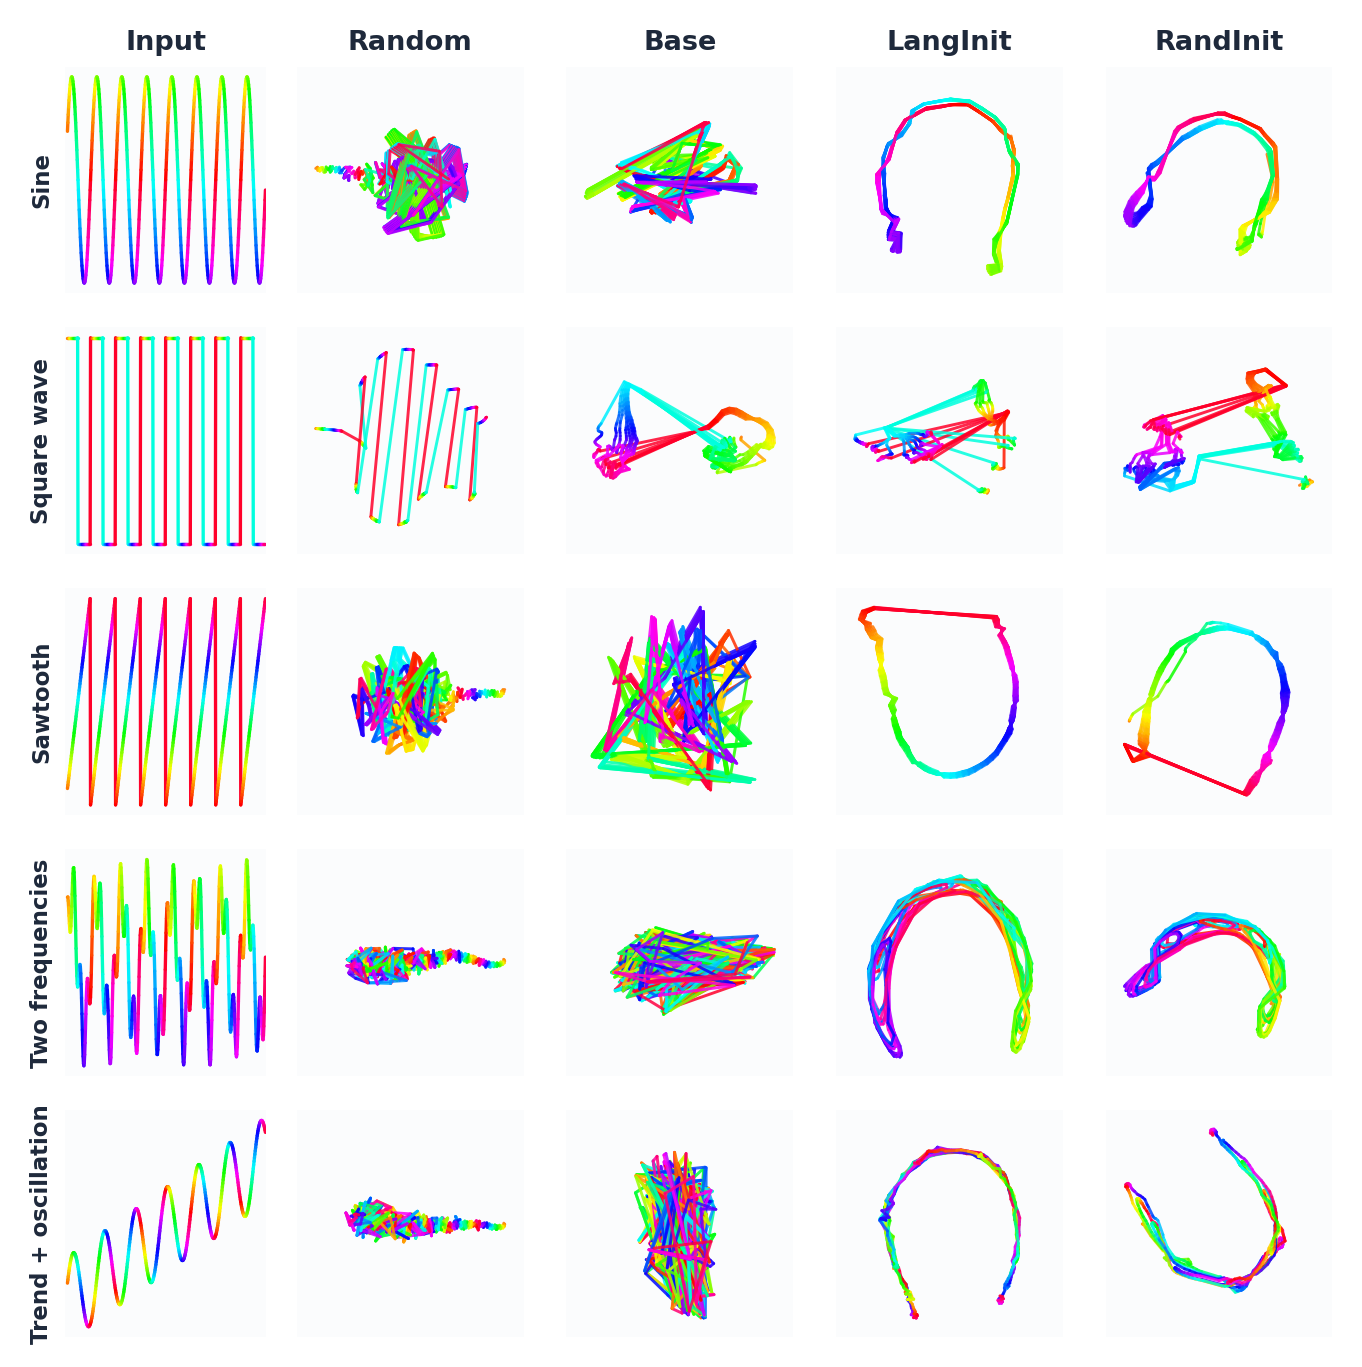
\includegraphics[width=0.85\textwidth]{figures/sec5/fig_synthetic_L13_tsne.png}
\caption{\textbf{Hidden-state trajectories for synthetic inputs at Layer~13 (t-SNE).} Same setup as Figure~\ref{fig:synthetic_pca} but using t-SNE (perplexity~30) instead of PCA. Despite the different global geometries revealed by PCA, t-SNE shows that LangInit and RandInit develop similar local neighborhood structure: periodic inputs form smooth, phase-ordered curves in both models, confirming that both arrive at functionally equivalent representations through different geometric paths.}
\label{fig:synthetic_tsne}
\end{figure}

\begin{figure}[!ht]
\centering
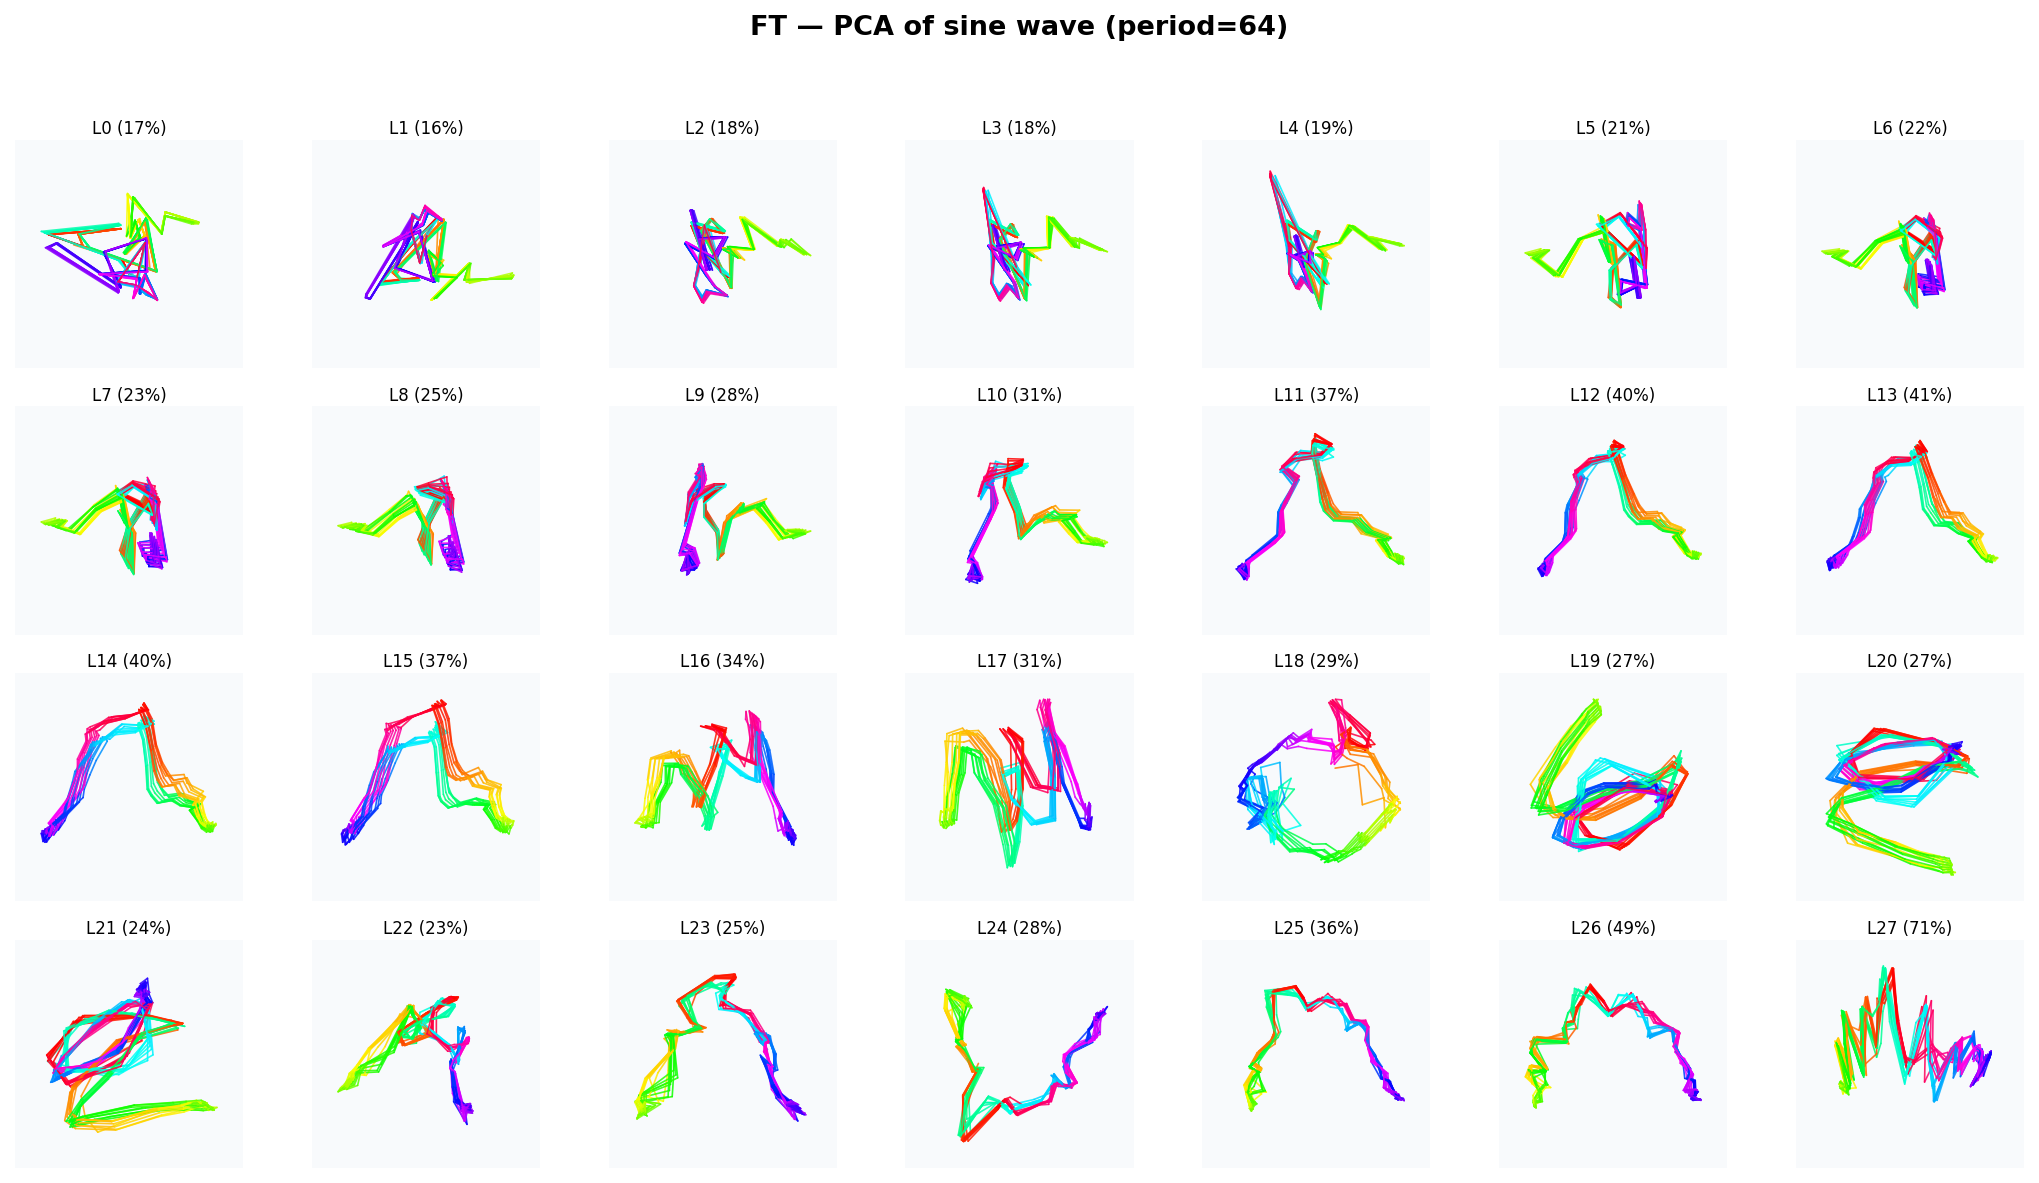
\includegraphics[width=\textwidth]{figures/sec5/fig_FT_pca_grid.png}
\caption{\textbf{LangInit: sine wave PCA trajectories across all 28 layers.} Each subplot shows the 2D PCA projection of hidden states from a sine wave (period~64) at one transformer layer, colored by input phase. Percentages show variance explained by 2 PCs. LangInit exhibits layer-specific geometry with varying complexity and moderate PCA variance (17--49\%), reflecting the rich, heterogeneous representations inherited from language pretraining.}
\label{fig:pca_grid_ft}
\end{figure}

\begin{figure}[!ht]
\centering
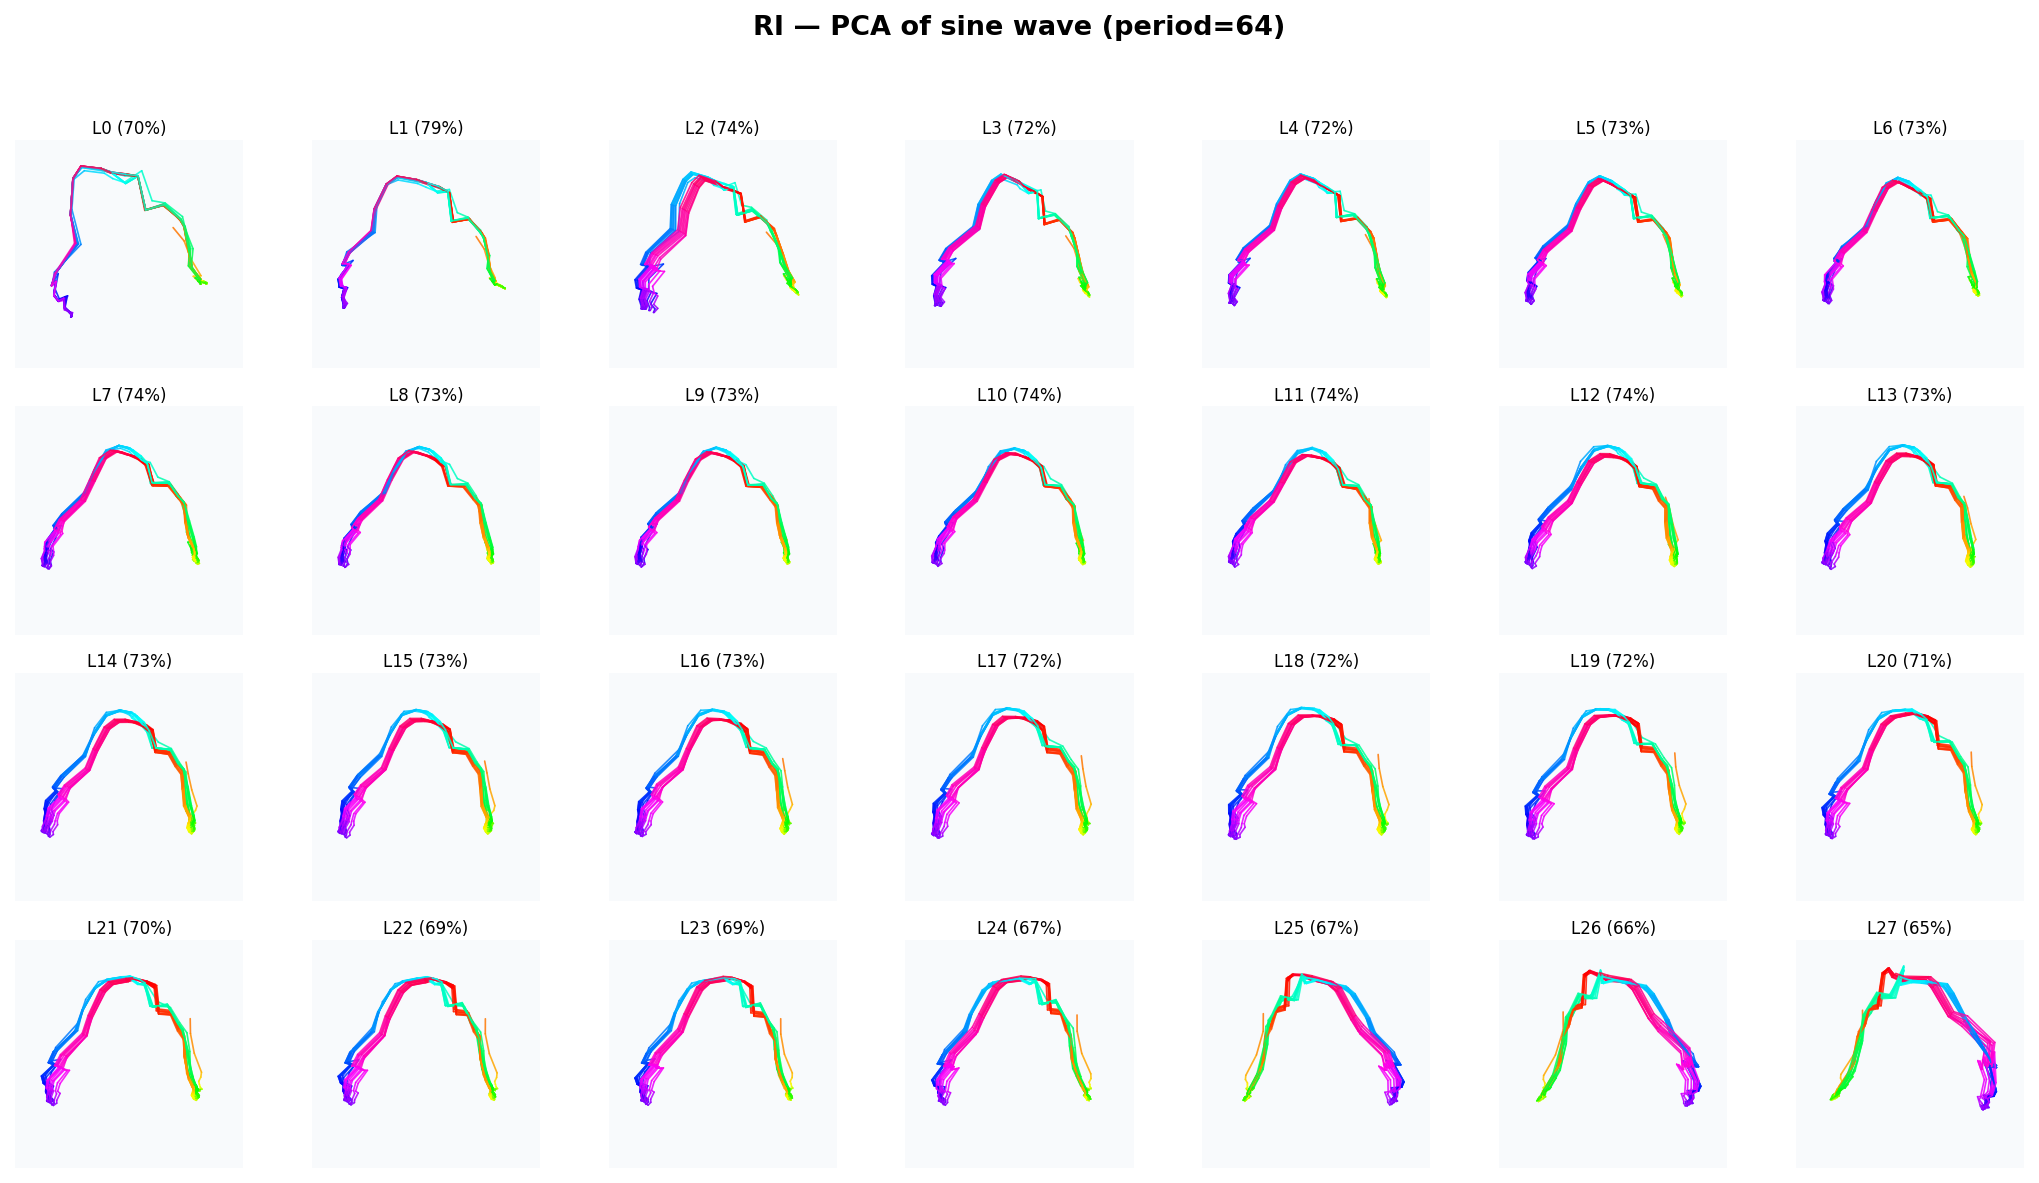
\includegraphics[width=\textwidth]{figures/sec5/fig_RI_pca_grid.png}
\caption{\textbf{RandInit: sine wave PCA trajectories across all 28 layers.} Same setup as Figure~\ref{fig:pca_grid_ft}. RandInit produces nearly identical clean arcs at every layer with uniformly high PCA variance (67--79\%), confirming that its learned representation is geometrically homogeneous across the network.}
\label{fig:pca_grid_ri}
\end{figure}

\begin{figure}[!ht]
\centering
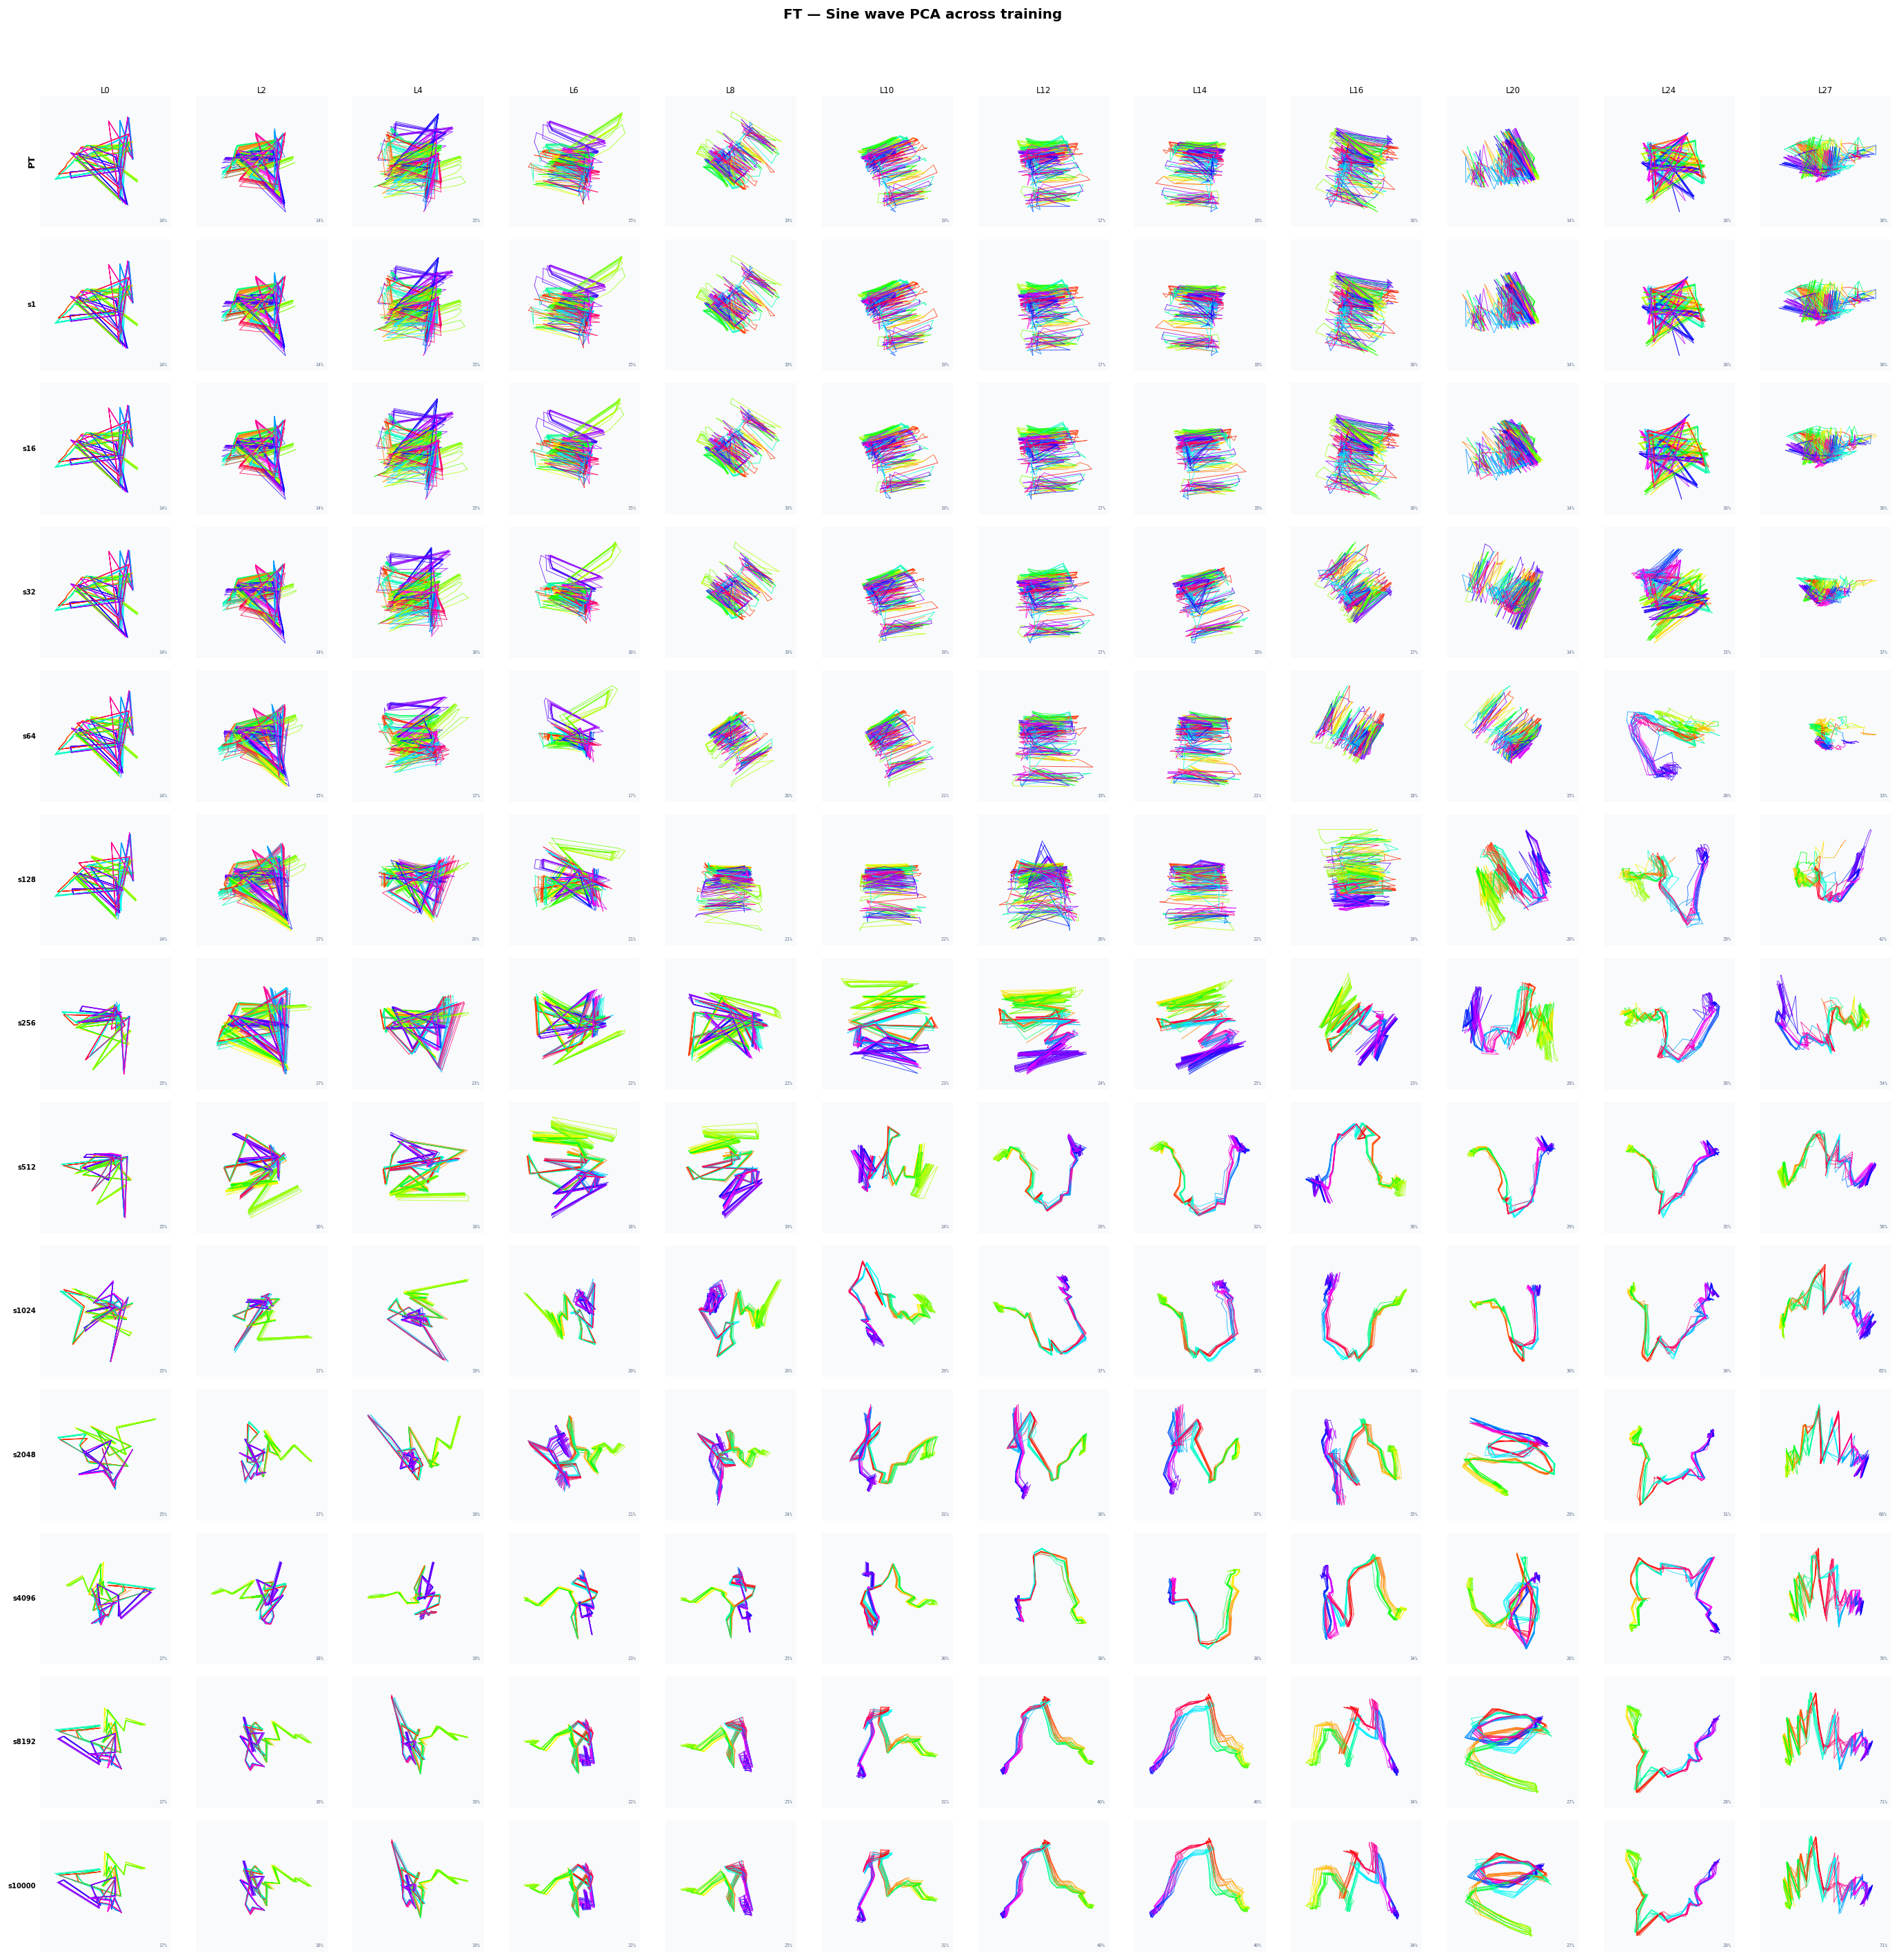
\includegraphics[width=\textwidth]{figures/sec5/fig_FT_evolution_grid.png}
\caption{\textbf{LangInit: sine wave representations across training checkpoints.} Rows are training steps (top: PT baseline; bottom: final checkpoint at step~10{,}000), columns are selected layers. LangInit begins from the pretrained model's complex trajectories and gradually reshapes them into structured loops, with the transition occurring around steps 256--1024.}
\label{fig:evolution_grid_ft}
\end{figure}

\begin{figure}[!ht]
\centering
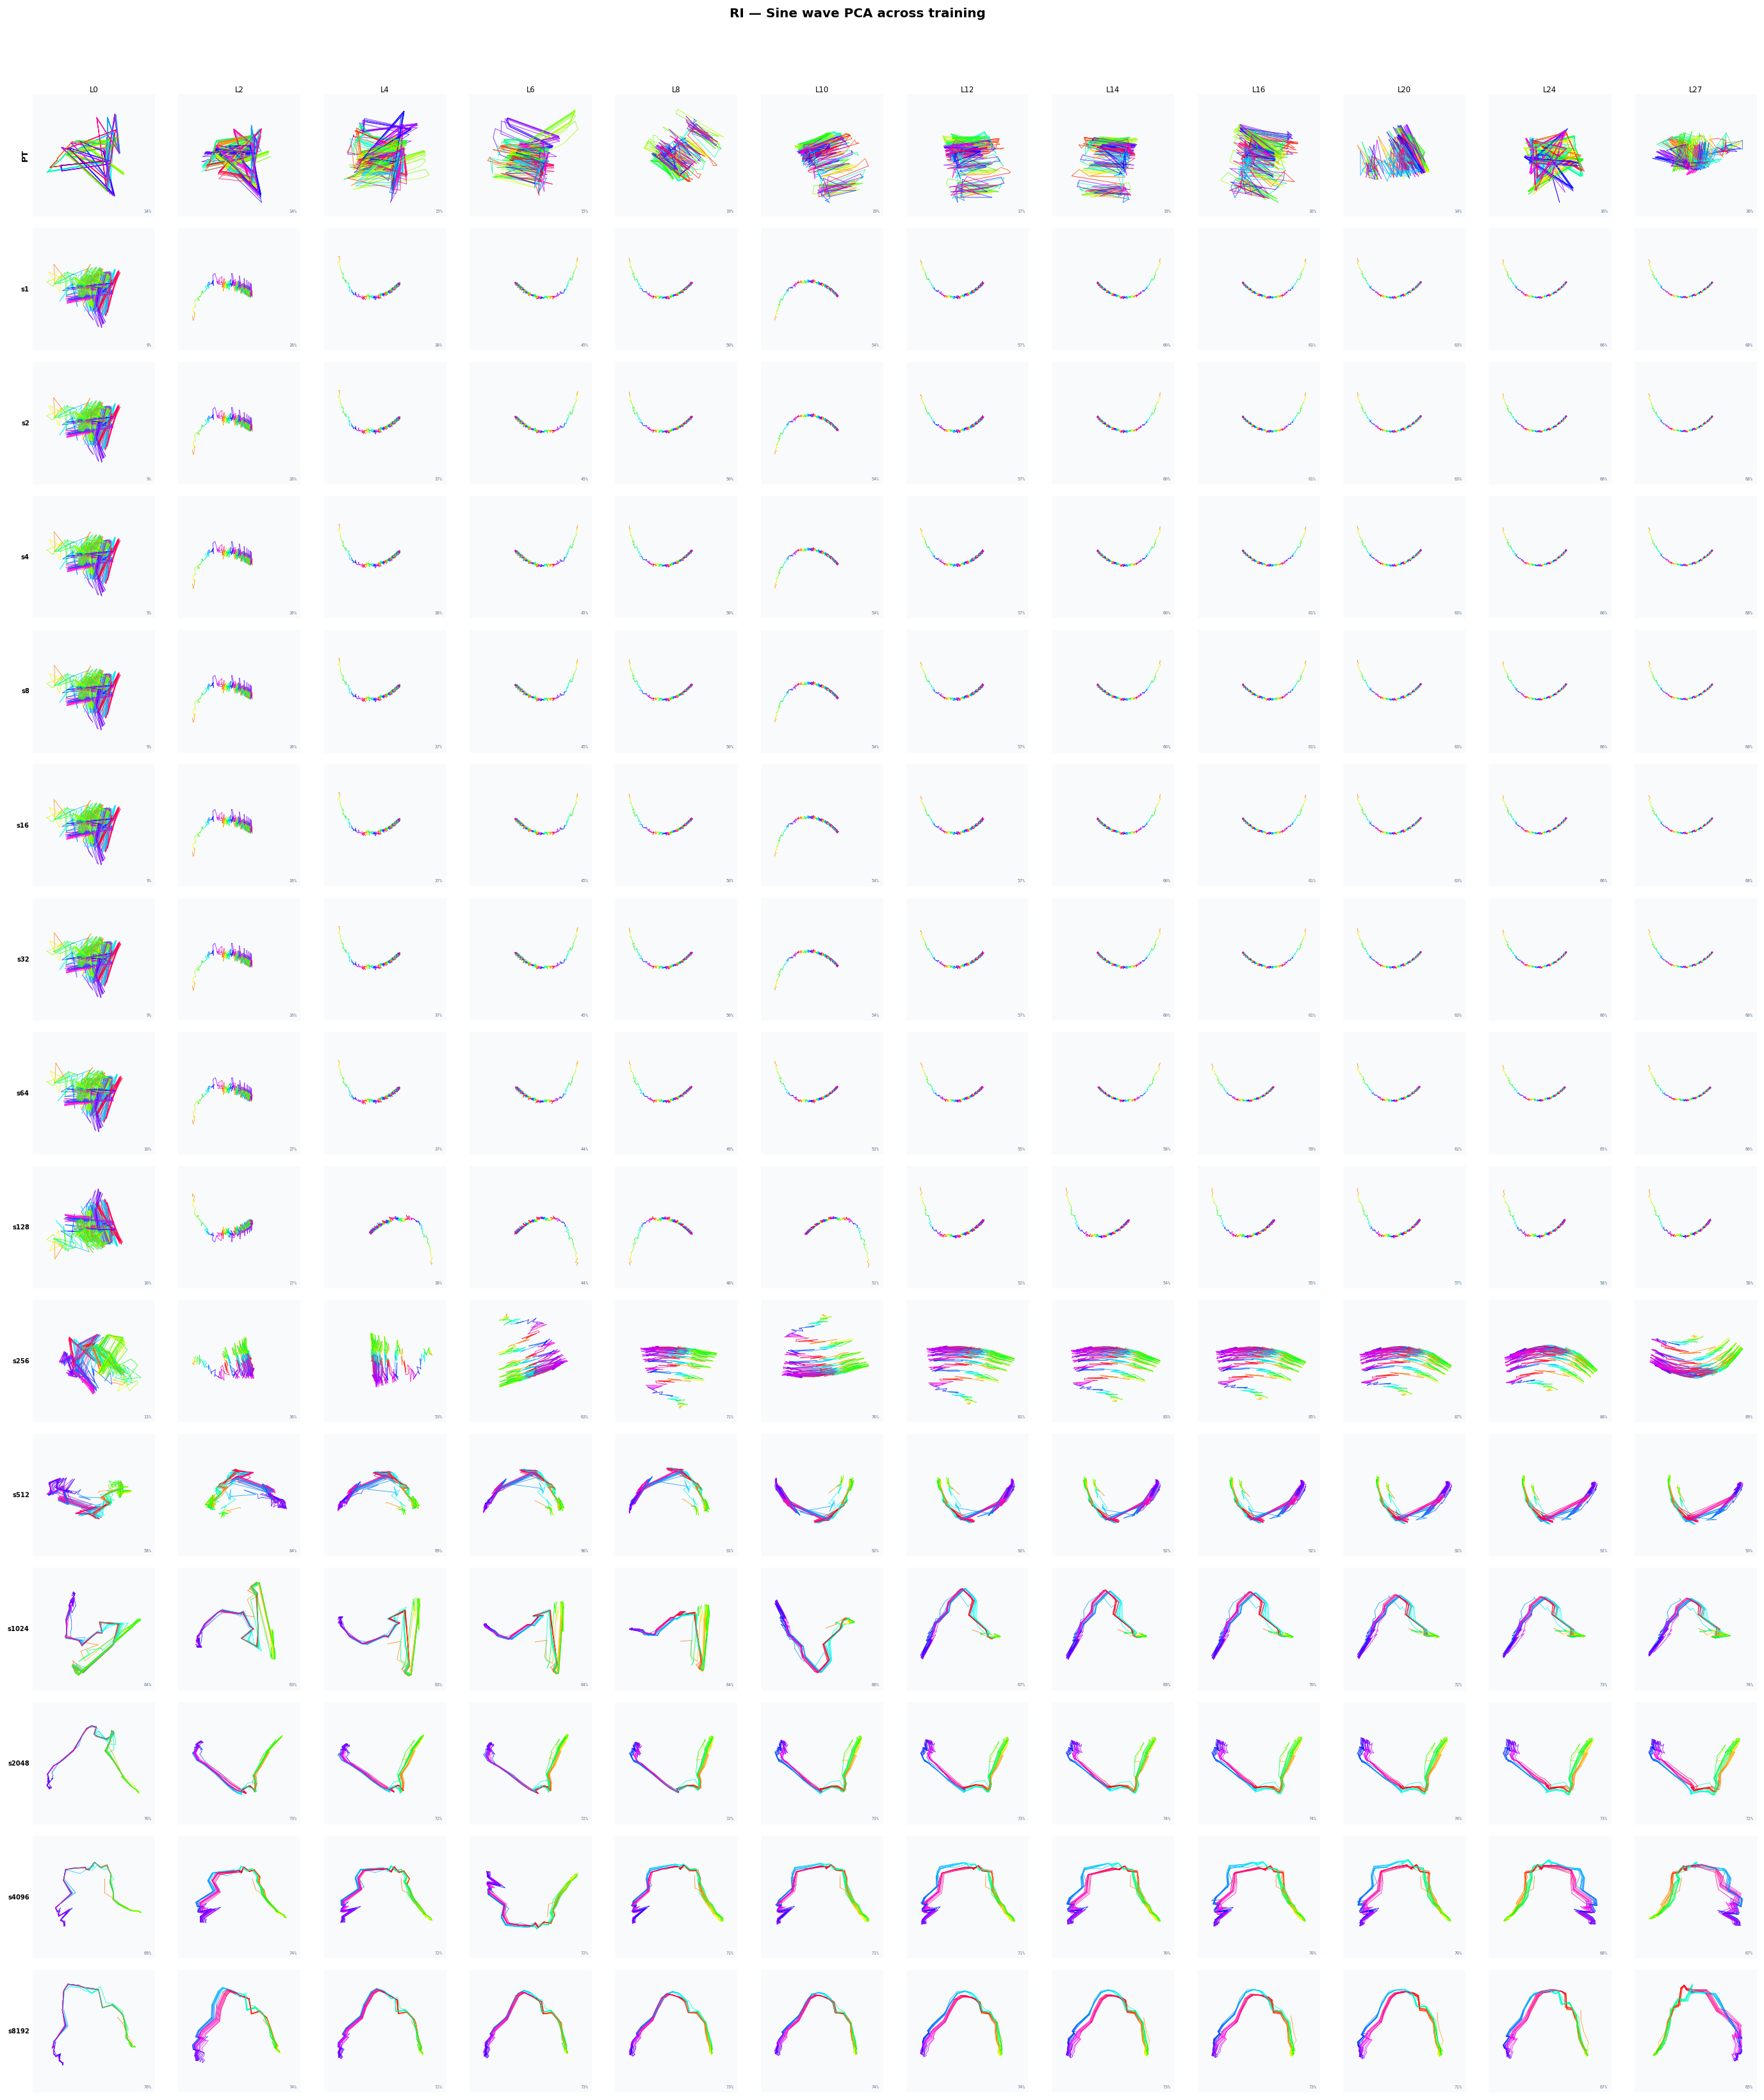
\includegraphics[width=\textwidth]{figures/sec5/fig_RI_evolution_grid.png}
\caption{\textbf{RandInit: sine wave representations across training checkpoints.} Same setup as Figure~\ref{fig:evolution_grid_ft}. RandInit starts from near-empty representations (random weights) and converges to uniform clean arcs by step~2048, with all layers collapsing to the same geometry simultaneously.}
\label{fig:evolution_grid_ri}
\end{figure}

\section{Causal Circuit Identification}
\label{app:circuit}

The correlational analyses in Section~\ref{sec:finetuning} show that finetuning reuses pretrained directions and that cross-domain features exist. Here we present a preliminary causal analysis: we identify specific model components responsible for periodic time-series prediction and test what role those components play in language modeling.

\subsection{Method}
\label{app:circuit_method}

Since FT\textsubscript{IO} only trains embedding and LM-head layers, its 28 transformer layers are identical to PT. We zero-ablate~\citep{wang2023interpretability} each of the 476 components (448 attention heads + 28 MLPs) on FT\textsubscript{IO} and measure the loss increase ($\Delta\mathcal{L}$) on periodic time series versus non-periodic controls.

\paragraph{Zero-ablation implementation.}
For each attention head, we register a \texttt{forward\_pre\_hook} on the output projection (\texttt{o\_proj}) that zeros the head's 128-dimensional slice of the concatenated 2048-dimensional head output before projection. For each MLP layer, we register a \texttt{forward\_hook} that replaces the MLP output with zeros, so the residual stream passes through unchanged. All ablations are performed under \texttt{torch.no\_grad()}.

\paragraph{Synthetic time series.}
We generate 20 windows (length 512) for each of nine synthetic types. \emph{Periodic}: sine, square wave, sawtooth, seasonal (trend + oscillation), damped sine. \emph{Control}: white noise, constant, linear trend, random walk. Each window is independently $z$-score normalized, clipped to $[-5, 5]$, and uniformly binned into 1024 tokens (matching the FT\textsubscript{IO} tokenizer). This yields 180 evaluation windows total (100 periodic, 80 control).

\paragraph{Selectivity metric.}
For each ablated component we compute:
\begin{align}
\Delta\mathcal{L}_\text{periodic} &= \bar{\mathcal{L}}_\text{ablated}^\text{periodic} - \bar{\mathcal{L}}_\text{baseline}^\text{periodic}, \\
\Delta\mathcal{L}_\text{control} &= \bar{\mathcal{L}}_\text{ablated}^\text{control} - \bar{\mathcal{L}}_\text{baseline}^\text{control}, \\
\text{selectivity} &= \Delta\mathcal{L}_\text{periodic} - \Delta\mathcal{L}_\text{control}.
\end{align}
Components with high $\Delta\mathcal{L}_\text{periodic}$ and high selectivity are specifically critical for periodic prediction rather than general-purpose.

\paragraph{Cumulative ablation.}
We compose multiple ablation hooks simultaneously using nested context managers. For the pairwise sweep, we test all $\binom{8}{2} = 28$ pairs of the top-8 selective components. For the growing cumulative, we add components one at a time in order of individual $\Delta\mathcal{L}_\text{periodic}$. The superadditivity ratio is $\rho = \Delta\mathcal{L}_\text{combined} / \sum_i \Delta\mathcal{L}_i^\text{individual}$~\citep{conmy2023automated, elhage2021mathematical}; we use a threshold of $\rho > 1.2$ to account for noise.

\paragraph{WikiText transfer.}
We ablate the top-5 circuit components simultaneously on 2{,}000 WikiText-103 passages (length 512) through the pretrained model (which shares identical transformer layers with FT\textsubscript{IO}). For each passage we record the per-sequence cross-entropy loss before and after ablation. The 50 most-degraded and 50 least-degraded passages are extracted for qualitative analysis.

\subsection{Results}

\paragraph{Individual component sweep.}
Table~\ref{tab:ablation_top} shows the top-8 components ranked by $\Delta\mathcal{L}_\text{periodic}$. The two most impactful are both in Layer~1: MLP\textsubscript{L1} ($\Delta\mathcal{L}_p = 5.75$, selectivity $= 3.44$) and head~L1H4 ($\Delta\mathcal{L}_p = 4.50$, selectivity $= 3.81$). Head~L20H0 is the third most impactful with the highest selectivity ($3.28$).

\begin{table}[h]
\centering
\caption{Top-8 components by $\Delta\mathcal{L}$ on periodic TS under zero-ablation. Selectivity $= \Delta\mathcal{L}_\text{periodic} - \Delta\mathcal{L}_\text{control}$ isolates periodicity-specific impact. Full sweep: 476 components.}
\label{tab:ablation_top}
\begin{tabular}{lrrr}
\toprule
Component & $\Delta\mathcal{L}_\text{periodic}$ & $\Delta\mathcal{L}_\text{control}$ & Selectivity \\
\midrule
MLP\textsubscript{L1}   & 5.75 & 2.31 & 3.44 \\
Head L1H4               & 4.50 & 0.69 & 3.81 \\
Head L20H0              & 3.40 & 0.13 & 3.28 \\
Head L13H6              & 3.35 & 2.56 & 0.79 \\
Head L23H6              & 2.00 & 0.06 & 1.94 \\
Head L21H8              & 1.85 & $-0.25$ & 2.10 \\
Head L15H3              & 1.55 & 0.38 & 1.18 \\
Head L11H8              & 1.25 & 0.56 & 0.69 \\
\bottomrule
\end{tabular}
\end{table}

\paragraph{Cumulative ablation reveals a composed circuit.}
The Layer~1 pair (head~L1H4 + MLP\textsubscript{L1}) is strongly superadditive: ablating them together produces $\Delta\mathcal{L}_p = 15.50$, which is 51\% larger than the sum of their individual effects ($\rho = 1.51$; Table~\ref{tab:cumulative}). No other pair among the 28 tested exceeds the $\rho > 1.2$ threshold. Adding head~L20H0 maintains superadditivity ($\rho = 1.36$); beyond three components, returns become subadditive ($\rho < 1$), indicating compensation rather than composition.

\begin{table}[h]
\centering
\caption{Cumulative ablation. The Layer~1 pair is strongly superadditive ($\rho = 1.51$); the core circuit saturates at 3 components.}
\label{tab:cumulative}
\begin{tabular}{lrrrr}
\toprule
Components & $\Delta\mathcal{L}_\text{periodic}$ & $\sum \Delta\mathcal{L}_\text{indiv.}$ & $\rho$ & $\Delta\mathcal{L}_\text{control}$ \\
\midrule
Head L1H4 + MLP\textsubscript{L1} & 15.50 & 10.25 & \textbf{1.51} & 2.38 \\
+ Head L20H0 (top-3)              & 18.55 & 13.65 & \textbf{1.36} & 3.69 \\
+ Head L21H8 (top-4)              & 18.40 & 15.50 & 1.19 & 3.06 \\
+ Head L23H6 (top-5)              & 18.55 & 17.50 & 1.06 & 3.00 \\
All top-8                          & 18.30 & 23.65 & 0.77 & 3.13 \\
\bottomrule
\end{tabular}
\end{table}

\paragraph{The periodicity circuit in language.}
We ablate the top-5 circuit components simultaneously on 2{,}000 WikiText-103 passages through the pretrained model. The circuit ablation causes a mean loss increase of $\Delta\mathcal{L} = 4.53$ nats---two orders of magnitude larger than any individual head's WikiText effect ($\leq 0.04$), confirming circuit-level interaction.

The most-degraded passages ($\Delta\mathcal{L} = 8$--$9$; Table~\ref{tab:wiki_full}) are dominated by sequential enumerations and repeating grammatical templates: biographical sequences (``married to\ldots she gave birth to\ldots''), game mechanics with parallel clause structure (``sets a task for each stage\ldots this task must be completed\ldots the player with the most''), Billboard chart progressions, award category listings, and structured Wikipedia sections with repeating headers. In contrast, the least-degraded passages ($\Delta\mathcal{L} < 2$) are dense, non-repetitive prose: ecclesiastical titles, academic citations, canonical law, and literary criticism---text where predicting the next token depends on semantic content rather than structural repetition.

This suggests the circuit tracks \emph{sequential repetitive structure}---the same abstract property shared by periodic time series and repetitive text. However, the evidence is preliminary: the WikiText passages most degraded by the circuit do not all show an obvious repetitive pattern, and disentangling the circuit's role in general sequence modeling from periodicity-specific computation requires further investigation.

\begin{table}[h]
\centering
\caption{WikiText-103 passages most and least degraded by ablation of the periodicity circuit (top-5 components). Mean $\Delta\mathcal{L} = 4.53$ across 2{,}000 passages.}
\label{tab:wiki_full}
\small
\begin{tabularx}{\textwidth}{r >{\raggedright\arraybackslash}X}
\toprule
$\Delta\mathcal{L}$ & Passage excerpt \\
\midrule
\multicolumn{2}{l}{\emph{Top 20 most degraded}} \\
9.19 & ``\ldots Townsend has been married to Tracy Turner, his girlfriend since he was 19. She gave birth to thei[r]\ldots'' \\
8.88 & ``\ldots Preston winger Will Hayhurst, a Republic of Ireland under-21 international, was signed on a one-month loan\ldots'' \\
8.88 & ``\ldots with the NHK Symphony Orchestra, but cancelled both deals upon Mwanga's return from Japan. Mwanga immediately quit\ldots'' \\
8.88 & ``\ldots his/her final score on the song, with money being awarded in Guitar Hero World Tour. The games have also added\ldots'' \\
8.75 & ``\ldots Viscount, sets a task for each stage. This task must be completed before the player can continue to another map\ldots'' \\
8.50 & ``\ldots The player character is Michel Ardan, an eccentric and intrepid French scientist who is enthusiastic, daring\ldots'' \\
8.38 & ``\ldots Best Music Video, Long Form. In 1998, the categories were retitled Best Short Form Music Video, and Best Long\ldots'' \\
8.31 & ``\ldots on the Billboard Hot 100 twenty-nine, the highest U.S. entry among all singles released from the album\ldots'' \\
8.31 & ``\ldots long run, with The A.V. Club attributing much of the show's early success to the character\ldots'' \\
8.25 & ``\ldots Yankovic recorded `Here's Johnny', a parody of `Who's Johnny' by El DeBarge. The song, a loving ode to\ldots'' \\
8.19 & ``\ldots The music video of `Crazy in Love', released in May 2003, was directed by Jake Nava and filmed\ldots'' \\
8.19 & ``\ldots Finishing with the worst record in the NHL, Columbus had the best chance of receiving the first overall pick\ldots'' \\
8.13 & ``\ldots while one in the Pyramid Texts says the name is based on words shouted by Osiris\ldots'' \\
8.06 & ``\ldots the album Daydream most resembles in its emphasis on R\&B grooves. Tucker specifically complimented `One Sweet Day'\ldots'' \\
8.00 & ``\ldots similar to Konami's Guitar Freaks and to a lesser extent Harmonix's previous music games such as Frequency\ldots'' \\
8.00 & ``\ldots he `hit the wall with play-along music games', and challenged the game makers to explore other ways\ldots'' \\
7.94 & ``\ldots saying that he `was upset. But when you see the talent that was there, it was an honour just to be in the final'\ldots'' \\
7.94 & ``\ldots Flags indicate national team as defined under FIFA eligibility rules. Players may hold more than one non-FIFA\ldots'' \\
7.94 & ``\ldots at the Television Critics Association summer media tour in Beverly Hills, California\ldots'' \\
7.94 & ``\ldots co-wrote and produced a song with Kenneth `Babyface' Edmonds, with whom she had collaborated on Music Box\ldots'' \\
\midrule
\multicolumn{2}{l}{\emph{Top 10 least degraded}} \\
0.83 & ``\ldots Porto e Santa Rufina; Sub-dean of the Sacred College of Cardinals; prefect of the S.C.\ of the Good Government\ldots'' \\
1.48 & ``\ldots Cardinal-Priest of SS.\ Giovanni e Paolo; Grand penitentiary; prefect of the Congregation for the correction\ldots'' \\
1.59 & ``\ldots From the Jewish Question to the Jewish State: An Essay on the Theory of Zionism (thesis), Princeton Univ.\ldots'' \\
1.77 & ``\ldots called Saprang's transfer a `demotion' and a `punishment.' However, Saprang himself claimed that he did not\ldots'' \\
1.82 & ``\ldots the Society of Jesus, provided he observed the canon law; and that it was desirable that the pope should\ldots'' \\
1.89 & ``\ldots the abnormal excess of white blood cells in people with the clinical syndrome described by Velpeau and Bennett\ldots'' \\
1.89 & ``\ldots The protagonist sounds like a `colonial administrator', and his reference to seeking a newer world echoes\ldots'' \\
1.94 & ``\ldots Mbaruk's nephew, Mbaruk bin Rashid, refused to acknowledge the appointment of a new leader\ldots'' \\
1.98 & ``\ldots 00 works were published underground over the course of the war. Literary discussions were held\ldots'' \\
2.02 & ``\ldots Although the poem was defended by a few critics, E.C. Pettet returned to the argument that the poem lacked\ldots'' \\
\bottomrule
\end{tabularx}
\end{table}

%%%%%%%%%%%%%%%%%%%%%%%%%%%%%%%%%%%%%%%%%%%%%%%%%%%%%%%%%%%%

\newpage
\section{Cross-Domain Feature Analysis via Crosscoders}
\label{app:crosscoder}

The circuit-level analysis in Appendix~\ref{app:circuit} shows that specific components are shared between time-series periodicity prediction and repetitive language modeling. Here we complement that \emph{component-level} analysis with a \emph{feature-level} analysis using crosscoders---sparse autoencoders with a shared encoder applied across domains---to discover individual latent features that fire on both time-series inputs and semantically coherent natural-language passages.

\subsection{Method}
\label{app:crosscoder_method}

\paragraph{Setup.}
We train one \emph{linear crosscoder} per transformer layer of Qwen3-0.6B.  Each crosscoder has a shared encoder $\mathbf{W}_{\mathrm{enc}} \in \mathbb{R}^{1024 \times 4096}$ followed by Top-$K$ sparsity ($K{=}64$), and two per-domain decoders $\mathbf{W}_{\mathrm{dec}}^{(\mathrm{PT})}, \mathbf{W}_{\mathrm{dec}}^{(\mathrm{FT})} \in \mathbb{R}^{4096 \times 1024}$ (12.6\,M parameters total, float32).  The encoder is applied independently to each domain's hidden states; because the weights are shared, the same latent feature can fire on both pretrained (PT) and fine-tuned (FT) inputs.

\paragraph{Domains.}
\emph{PT}: Time series formatted as space-separated decimal strings (e.g., \texttt{0.123 -0.456 1.789\,\ldots}), tokenized by the Qwen3-0.6B tokenizer.  Sub-tokens corresponding to each timestep value are mean-pooled to produce one $1024$-dim vector per timestep.
\emph{FT}: The same time series normalized per-window ($z$-score), clipped to $[-5,5]$, and uniformly binned into 1024 tokens for the fine-tuned model.

\paragraph{Training.}
Input: 3{,}000 windows ($T{=}512$) from GiftEval~\citep{aksu2024giftevalgeneralizedinstructionfollowing}, precomputed as memory-mapped hidden-state arrays.  Loss: per-domain MSE between normalized inputs and decoder reconstructions, summed over PT and FT.  Dead-feature recovery (AuxK; top-64 among features firing ${<}1$\% over the last 1{,}000 steps, weight $\frac{1}{32}$, active after step 1{,}000).  AdamW, $\mathrm{lr}{=}3{\times}10^{-4}$, 500 warmup steps, cosine decay over 10{,}000 steps.  Early stopping after 1{,}500 steps without validation improvement (minimum step 2{,}000).

\paragraph{Feature analysis pipeline.}
After training, 50{,}000 time-series windows are encoded; for each of the 4{,}096 features we record the PT and FT firing rates (fraction of windows with non-zero activation).  Features firing ${\geq}1$\% in both domains are labeled \textsc{PT\_FT} and ranked by $\text{balance} = \min(\text{rate}_{\mathrm{PT}}, \text{rate}_{\mathrm{FT}})$.  For the top-30 balanced features, we extract the 10 highest-activating time-series windows and 10 highest-activating WikiText-103 passages (30{,}000 sequences, 512 tokens each, encoded through the PT model and the shared crosscoder encoder with separate normalization statistics).

\subsection{Results}
\label{app:crosscoder_results}

Layers 7--10 are the sweet spot for shared cross-domain features (Table~\ref{tab:crosscoder_balance}).  Early layers (0, 6) and late layers (13, 20) show almost no balanced features.  Below we present four features with the clearest cross-domain links: each fires on a specific time-series pattern \emph{and} on thematically coherent WikiText passages.

\begin{table}[h]
\centering
\caption{Cross-layer feature balance.  ``Best balance'' is the highest $\min(\text{rate}_\text{PT}, \text{rate}_\text{FT})$ among all 4{,}096 features.  Layers~7--10 concentrate almost all balanced features.}
\label{tab:crosscoder_balance}
\small
\begin{tabular}{rrrr}
\toprule
Layer & Best balance & \# Features ${>}30$\% bal.\ & Train loss \\
\midrule
0  & 2.1\%  & 0  & 0.016 \\
6  & 29.4\% & 0  & 0.050 \\
\textbf{7}  & \textbf{57.0\%} & \textbf{10} & 0.052 \\
\textbf{8}  & \textbf{52.1\%} & \textbf{6}  & 0.062 \\
\textbf{9}  & \textbf{51.2\%} & \textbf{7}  & 0.067 \\
\textbf{10} & \textbf{55.7\%} & \textbf{5}  & 0.057 \\
11 & 47.1\% & 4  & 0.062 \\
12 & 47.9\% & 3  & 0.062 \\
13 & 50.0\% & 1  & 0.059 \\
20 & 2.0\%  & 0  & 0.120 \\
\bottomrule
\end{tabular}
\end{table}

%% --- Feature A: Quantitative magnitude transitions ---

\paragraph{Feature 1712 (Layer~10) --- Quantitative magnitude transitions.}
PT firing rate: 50.4\%, FT: 41.8\%, WikiText: 14.1\%.  This feature detects step changes and regime shifts in time series---values that jump from a near-zero baseline to a sustained high plateau---and fires on text passages dense with numerical measurements and unit conversions (Figure~\ref{fig:crosscoder_magnitude}).

\begin{figure}[h]
\centering
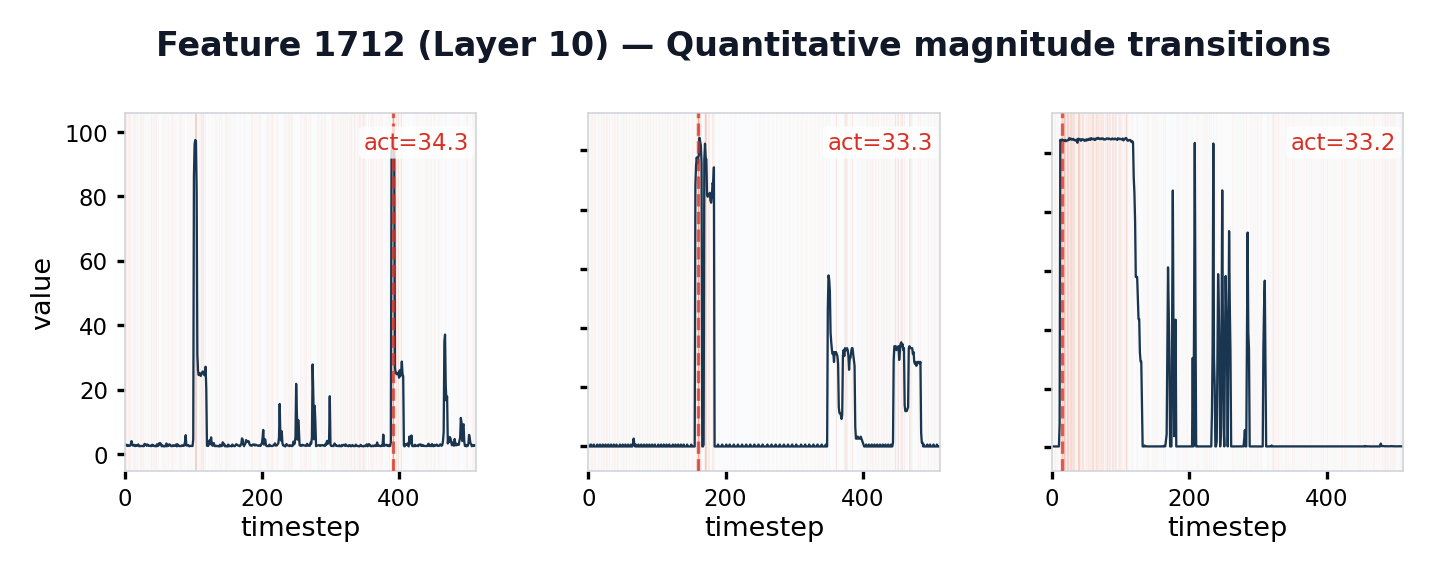
\includegraphics[width=\textwidth]{figures/appendix/fig_crosscoder_magnitude.png}
\caption{\textbf{Feature~1712 (Layer~10): Quantitative magnitude transitions.}  Top-3 activating time-series windows.  Blue: raw signal; red dashed: peak-activation timestep; orange shading: activation intensity.  All three windows share a sudden jump from a low baseline to a high-magnitude plateau.}
\label{fig:crosscoder_magnitude}
\end{figure}

Top-5 WikiText passages at the peak-activation token:
\begin{enumerate}[nosep, leftmargin=1.5em]
\item \emph{(act=14.1)} ``\ldots becoming later in the year by about two days every 243-year cycle.  Transits usually occur in pairs, on nearly the same date eight years apart.''
\item \emph{(act=13.8)} ``In practice, forward premiums and discounts are quoted as annualized percentage deviations from the spot exchange rate\ldots''
\item \emph{(act=13.7)} ``Wages are reflective of the type of jobs available locally, including higher than average employment in manufacturing and the public sector.  The working age population of the town in 2011\ldots''
\item \emph{(act=13.7)} ``So for americium-241, the resistivity at 4.2\,K increases with time from about 2\,\textmu Ohm$\cdot$cm to 10\,\textmu Ohm$\cdot$cm after 40 hours, and saturates at about 16\,\textmu Ohm$\cdot$cm\ldots''
\item \emph{(act=13.7)} ``Falcon's Fury can theoretically accommodate 800 riders per hour.  Carbon-fiber wings buttress each end of a group of seats\ldots''
\end{enumerate}
The shared representation encodes \emph{quantitative magnitude and transition}: literal level shifts in time series, and passages dense with measurements, unit conversions, and numerical comparisons in text.

%% --- Feature B: Tropical weather systems ---

\paragraph{Feature 2469 (Layer~9) --- Tropical weather systems.}
PT: 29.9\%, FT: 20.7\%, WikiText: 12.6\%.  Fires on volatile, regime-switching time series and exclusively on tropical cyclone and hurricane narratives in text (Figure~\ref{fig:crosscoder_weather}).

\begin{figure}[h]
\centering
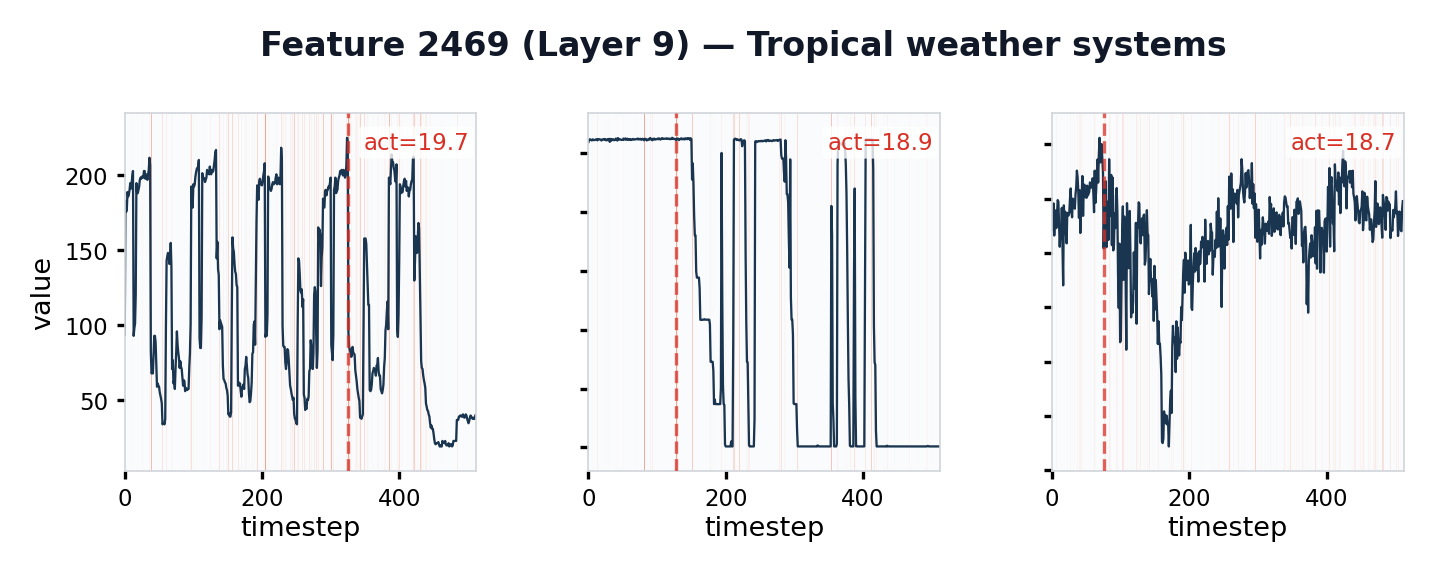
\includegraphics[width=\textwidth]{figures/appendix/fig_crosscoder_weather.png}
\caption{\textbf{Feature~2469 (Layer~9): Tropical weather systems.}  Top-3 activating windows.  The left window shows high-variance oscillations with abrupt drops; the middle and right show diverse volatile patterns with regime switching.}
\label{fig:crosscoder_weather}
\end{figure}

Top-5 WikiText passages:
\begin{enumerate}[nosep, leftmargin=1.5em]
\item \emph{(act=8.7)} ``\ldots the mean locus of formation shifts westward to the Caribbean and Gulf of Mexico, reversing the eastward progression of June through August.  Wind shear from westerlies increases substantially through November\ldots''
\item \emph{(act=8.3)} ``\ldots due to a combination of very high wind shear and dry air.  By October~17, most of the deep convection associated with the system dissipated; however, a brief decrease in wind shear allowed Omar to re-strengthen\ldots''
\item \emph{(act=8.1)} ``The wave continued westward and related thunderstorm activity increased during the following week.  The convective system organized into Tropical Depression Twenty-E on September~28\ldots''
\item \emph{(act=8.1)} ``A tropical wave moved across the northeast Pacific Ocean and formed a tropical depression south of Mexico on October~16.  It strengthened at a moderate pace and reached hurricane intensity on October~18.''
\item \emph{(act=7.9)} ``\ldots formation of Typhoon Chanchu in the western Pacific enhanced convective activity over the Bay of Bengal.  By April~22, a trough developed along an axis from the southern Bay of Bengal eastward to the Andaman Sea.''
\end{enumerate}
The time-series patterns---volatile signals with sudden regime changes---mirror the physical phenomena described in the text: tropical storms that intensify, weaken under wind shear, and shift track.

%% --- Feature C: Naval battle events ---

\paragraph{Feature 3888 (Layer~7) --- Naval battle events.}
PT: 18.5\%, FT: 26.3\%, WikiText: 10.5\%.  Fires on sharp isolated spikes in otherwise stable time series and on naval/military battle narratives with precise timestamps (Figure~\ref{fig:crosscoder_naval}).

\begin{figure}[h]
\centering
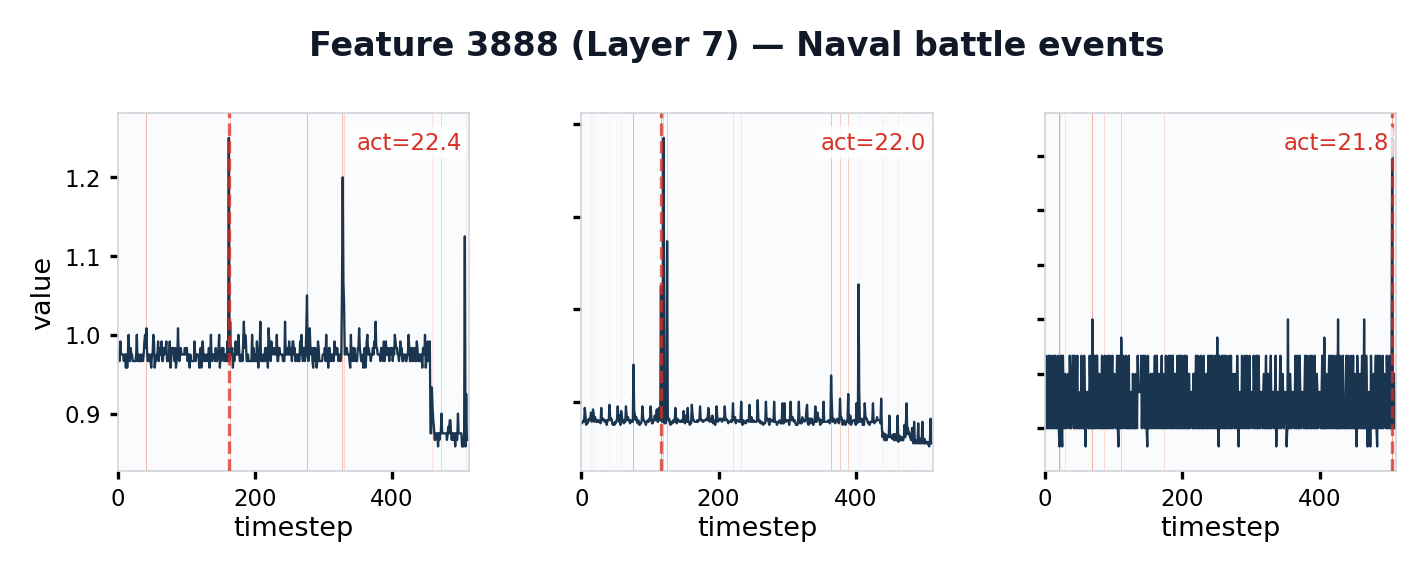
\includegraphics[width=\textwidth]{figures/appendix/fig_crosscoder_naval.png}
\caption{\textbf{Feature~3888 (Layer~7): Naval battle events.}  Top-3 activating windows.  Each shows a low-variance baseline punctuated by sharp spikes at the peak-activation timestep (red dashed line).}
\label{fig:crosscoder_naval}
\end{figure}

Top-5 WikiText passages:
\begin{enumerate}[nosep, leftmargin=1.5em]
\item \emph{(act=10.1)} ``King George V had only 32 percent of her fuel left while Rodney had only enough fuel to continue the chase at high speed until 8:00 the following day.  Admiral Tovey signalled his battlegroup\ldots''
\item \emph{(act=9.3)} ``At 7:20 on 19~July, the destroyer force spotted and was spotted by a pair of Italian light cruisers; Giovanni dalle Bande Nere and Bartolomeo Colleoni, which opened fire seven minutes later.''
\item \emph{(act=9.2)} ``Shortly before 16:00 the battlecruisers of I~Scouting Group encountered the British 1st Battlecruiser Squadron under the command of Vice Admiral David Beatty.  The opposing ships began an artillery\ldots''
\item \emph{(act=9.2)} ``The eastern wind was not communicated to the aircraft, but was 270\textdegree, varying from 20 to 40~knots (37 to 74~km/h).  The take-off started at 14:42:43\ldots''
\item \emph{(act=9.1)} ``\ldots torpedo boat attacks and at 07:30, Burrough sent Eskimo and Somali back to help Manchester but they arrived too late, took on survivors\ldots''
\end{enumerate}
Both modalities encode \emph{sudden, precisely-located events}: an anomalous spike at a single timestep in time series, and a precisely-timestamped combat event in text.

%% --- Feature D: Missing / null data ---

\paragraph{Feature 2567 (Layer~8) --- Missing / null data.}
PT: 35.9\%, FT: 36.8\%, WikiText: 9.4\%.  This feature fires exclusively on NaN/missing time-series data (all 10 top-activating windows are entirely NaN, with peak activation 40.3) and on \texttt{<unk>} tokens and incomplete references in text.

Top-5 WikiText passages:
\begin{enumerate}[nosep, leftmargin=1.5em]
\item \emph{(act=19.8)} ``\ldots at the Royal Navy School of Flight Deck Operations at RNAS Culdrose.  The following is an incomplete list of some of the surviving aircraft.''
\item \emph{(act=18.5)} ``\texttt{<unk>}, \texttt{<unk>}, \texttt{<unk>}, \texttt{<unk>}, \texttt{<unk>}, Ulaid.  Slightly later major groups included the Connachta, \texttt{<unk>}, \texttt{<unk>}.  Smaller groups included the \texttt{<unk>}\ldots''
\item \emph{(act=18.0)} ``\ldots he encountered bad weather, forcing him to return to Japan with heavy damage.  Without waiting for Vizcaino, another ship---built in Izu by the Tokugawa shogunate\ldots''
\item \emph{(act=17.8)} ``Luke 9: \texttt{<unk>}-\texttt{<unk>} --- $\kappa\alpha\grave{\iota}$ \texttt{<unk>}, \texttt{<unk>} \texttt{<unk>} \texttt{<unk>} $\pi\nu\varepsilon\acute{\upsilon}\mu\alpha\tau o\varsigma$ \texttt{<unk>} \texttt{<unk>}\ldots''
\item \emph{(act=17.7)} ``\ldots whom he married in the late 250s when she was 17 or 18 years old.  The number of children Odaenathus had with his first wife is unknown and only one is attested.''
\end{enumerate}
The model represents \emph{absent information} identically across modalities: NaN values in time series and \texttt{<unk>} tokens in text both occupy the same region of representation space.

\subsection{Discussion}

The crosscoder analysis reveals that layers~7--10 contain specific, thematically coherent features shared between time-series and language representations.  The most interpretable features tend to have moderate balance (15--45\%) rather than the highest balance ($>$50\%), which corresponds to generic backbone features.  The four features documented above encode distinct representational primitives---\emph{quantitative magnitude transitions}, \emph{volatile regime switching}, \emph{punctual disruption}, and \emph{absent information}---that manifest as both time-series patterns and specific text genres.

This complements the circuit-level finding from Appendix~\ref{app:circuit}: the periodicity circuit's components operate at specific layers (L1, L20), while the crosscoder features are concentrated in the intermediate layers (7--10) where the PT and FT representations are most aligned.  Together, these analyses suggest that LangInit exploits both circuit-level and feature-level structure from language pretraining when processing time series.

%%%%%%%%%%%%%%%%%%%%%%%%%%%%%%%%%%%%%%%%%%%%%%%%%%%%%%%%%%%%

\newpage
CHECKLIST TODO
% \input{checklist.tex}


\end{document}